\chapter{VECTOR ALGEBRA}

\begin{definition}
A vector is defined as a physical quantity having magnitude and a direction associated with it. 
\end{definition}
\begin{example}
	 Displacement,Velocity, Acceleration, Force ,Torque,Angular momentum etc. 
\end{example}
\section{Vector representation}
Geometrically  a  vector  is  represented  by  a  directed  line  segment, with length proportional to the magnitude.The direction of the arrow gives the direction of the vector.\newline
We will refer to the start of the arrow as the tail and the end as the tip or head. The vector between two points P and Q  will be denoted as, $\overrightarrow{\mathrm{P Q}}$(or by a boldface $\mathbf{PQ}$). And the  magnitude as $|\mathrm{ PQ}| .$  Magnitude will also be called length or norm.\\\\ Analytically a three  dimensional  vector  can  be  specified  by  an  ordered  set  of  three  numbers,  called  its  components.The magnitude  of  the  components  depend  on  the  coordinate  system  used. (A vector can be extended to $n$ dimensions). A vector $\vec{A}$ is represented by $\left(A_{x}, A_{y}, A_{z}\right)$ in cartesian (rectangular) coordinate system .\\Magnitude of vector $\vec{\mathrm A}$ is given by, $|\vec{\mathrm A}|=\sqrt{\mathrm A_{x}^{2}+\mathrm A_{y}^{2}+\mathrm A_{z}^{2}}$
\subsection{Position vector:} 
\begin{definition}
	Vectors that start at the origin and terminate at any arbitrary point are called position vectors. These are used to determine the position of a point with reference to the origin.
\end{definition}
\begin{figure}[H]
	\centering
	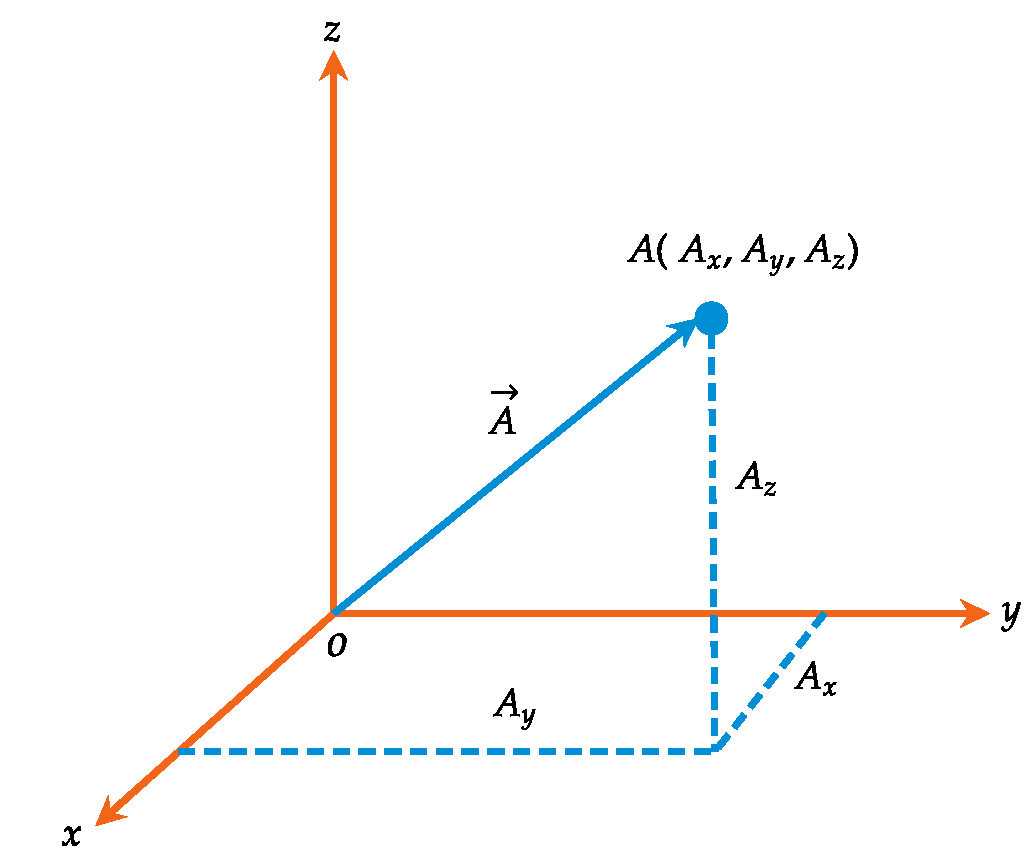
\includegraphics[width=0.4\textwidth]{vector2}
	\caption{Representation of position vector $\vec{A }$}
\end{figure}
 Any vector $\vec{\mathrm A}$ in the $3-\mathrm{\mathrm D}$ right handed rectangular cartesian coordinate system can be represented as,
 \begin{equation}
$$\vec{\mathrm A}=\mathrm A_{x} \hat{i}+\mathrm A_{y} \hat{j}+\mathrm A \hat{k}$$
 \end{equation} 
Where, $\hat{i}, \hat{j}$ and $\hat{k}$ are the unit vectors in direction of $x, y$ and $z$ axis respectively. $\mathrm A_{x}, \mathrm A_{y} $ and $ \mathrm A_{z}$ are the
cartesian components or projections of vector $\vec{A}$ along $x, y, z$ axis.
 \begin{exercise}
	 If $\mathrm A$ and $\mathrm B$ are (3,4,5) and $(6,8,9),$ find $\vec {\mathrm {A B}}$.
	\end{exercise}
\begin{answer}
$$\begin{aligned} \overrightarrow{\mathrm {A B}} &=\text { Position vector of } \mathrm B-\text { Position vector of } \mathrm A \\ &=(6 \hat{i}+8 \hat{j}+9 \hat{k})-(3 \hat{i}+4 \hat{j}+5 \hat{k}) \\ &=3 \hat{i}+4 \hat{j}+4 \hat{k} \end{aligned}$$
\end{answer}

\subsection{Unit vector:} 
\begin{definition}
	A vector quantity having unit magnitude is called unit vector.A unit vector along $\vec{A}$ is defined as,
	\\$\hat{\mathrm A}=\frac{\vec{\mathrm A}} {|\vec{\mathrm A}|}=\frac {\left(\mathrm A_{x} \hat{i}+\mathrm A_{y} \hat{j}+\mathrm A_{z} \hat{k}\right) } {\sqrt{\mathrm A_{x}^{2}+\mathrm A_{y}^{2}+\mathrm A_{z}^{2}}}$
\end{definition}
 \begin{exercise}
 	Find unit vector in the direction of vector $\vec{a}=2 \hat{i}+3 \hat{j}+\hat{k}$
 	 \end{exercise}
  \begin{answer}
  	
  	\begin{align*}
  		\text{Magnitude of }\vec{ a}&=\sqrt{2^{2}+3^{2}+1^{2}}\\
  		|\vec{a}|&=\sqrt{4+9+1}=\sqrt{14}\\
  		\text{Unit vector in direction of }\vec{a}&=\frac{\vec{a}}{| \vec{a}|}\\
  		\hat{a}&=\frac{1}{\sqrt{14}}[2 \hat{i}+3 \hat{j}+1 \hat{k}] \\
  		\hat{a}&=\frac{2}{\sqrt{14}} \hat{i}+\frac{3}{\sqrt{14}} \hat{i}+\frac{1}{\sqrt{14}} \hat{k}
  	\end{align*}
  	
  \end{answer}
  \subsection{Direction cosines}
In analytical geometry the direction cosines are the angles made by the vector with  the three coordinate axes.\\\\\textbf{Direction cosines of vector $\vec{\mathrm A}$} :
\\\newline If $\vec{\mathrm A}$ makes angles $\alpha, \beta, \gamma$ with $x, y$ and $z$ axes respectively, then direction cosines of $\vec{\mathrm A}$ are defined as,
\begin{minipage}{0.6\textwidth}
	\begin{flalign*}
	&l=\cos \alpha=\frac{\mathrm A_{x}}{\mathrm A}\quad ;\quad  m=\cos \beta=\frac{\mathrm A_{y}}{\mathrm A} \quad ;\quad  n=\cos \gamma=\frac{\mathrm A_{z}}{\mathrm A} \\  &l^{2}+m^{2}+n^{2}=1\\\\
	&\text{Then the unit vector along } \vec{\mathrm A}\text{ can be written as,}\\
	& \hat{\mathrm A}=l \hat{i}+m \hat{j}+n \hat{k}\\
	\end{flalign*}
\end{minipage}
\begin{minipage}{0.4\textwidth}
	\begin{figure}[H]
		\centering
		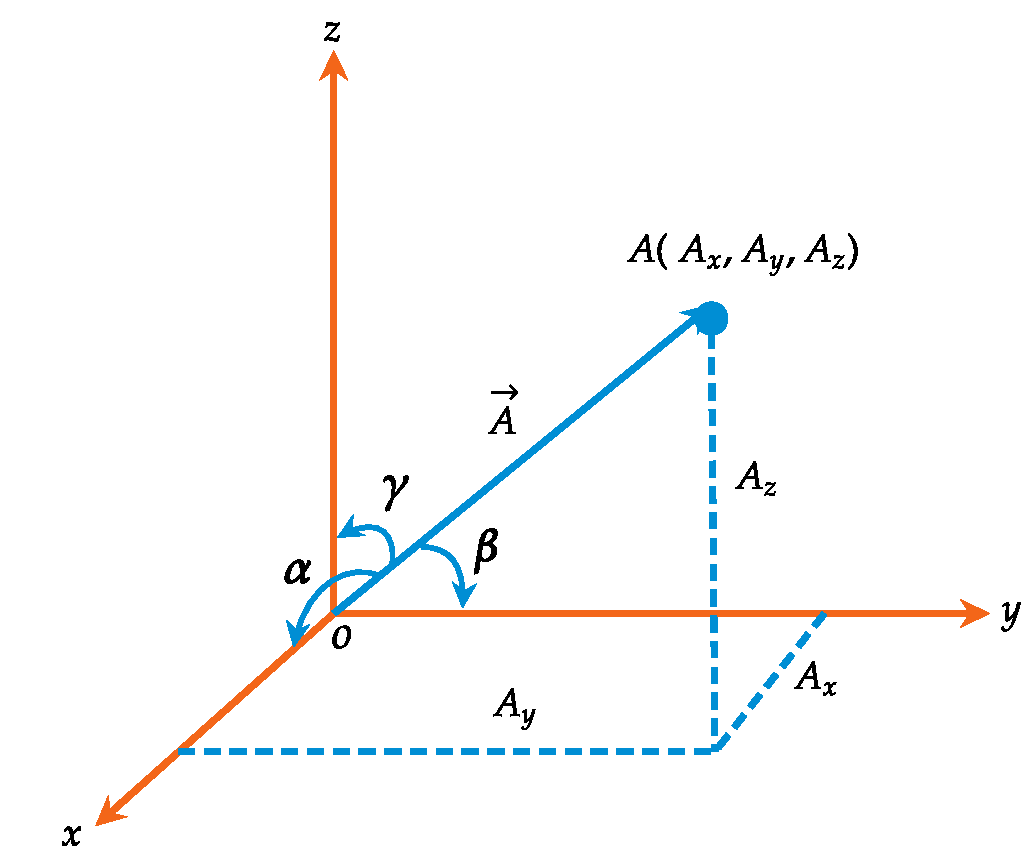
\includegraphics[width=6cm,height=6cm]{direction cosine}\caption{Direction cosine.}
	\end{figure}
\end{minipage}
\section{Types of vectors}
\begin{itemize}
	\item \textbf{{Equal vectors}}\hspace{0.74cm}\textbf{:}\quad Vectors having same magnitude and same direction.
	\item \textbf{Null Vectors }\hspace{0.82cm}\textbf{:} \quad Vectors having coincident initial and terminal point i.e its magnitude is zero and it has any arbitrary direction.
	\item \textbf{Reciprocal Vector }\textbf{:}\quad Vector having same direction as $\vec{\mathrm  A}$ but magnitude reciprocal to that of $\vec{\mathrm A},$ is known as the reciprocal vector of $\mathrm A$ Reciprocal vector of $\vec{\mathrm A}$ is $\vec{\mathrm A}-\frac{1}{\mathrm A} \hat{\mathrm A}$.
	\item \textbf{Negative Vector}\hspace{0.3cm} \textbf{:}\quad Vectors having same magnitude as $\vec{\mathrm a}$ but direction opposite to that of $\vec{\mathrm A},$ is known
	as the negative vector of $\vec{\mathrm a} .$ Negative vector as $\vec{\mathrm A}$ is $-\vec{\mathrm A}=-|\mathrm A| \hat{\mathrm A}$.
\end{itemize}
\section{Vector operations}\index{Vector operations}
\subsection{Vector addition}
\begin{itemize}
	\item 	\textbf{Triangular law of vector addition:}
	\begin{itemize}
		\item Place the tail of $\vec{\mathrm A}$ at the head of $\vec{\mathrm B} $.
		\item The resultant vector $\vec{\mathrm A}+\vec{\mathrm B}$ is formed by connecting the tail of the first vector to the head of the last vector. 
	\end{itemize}
\begin{figure}[H]
	\begin{minipage}{0.45\textwidth}
		\centering
		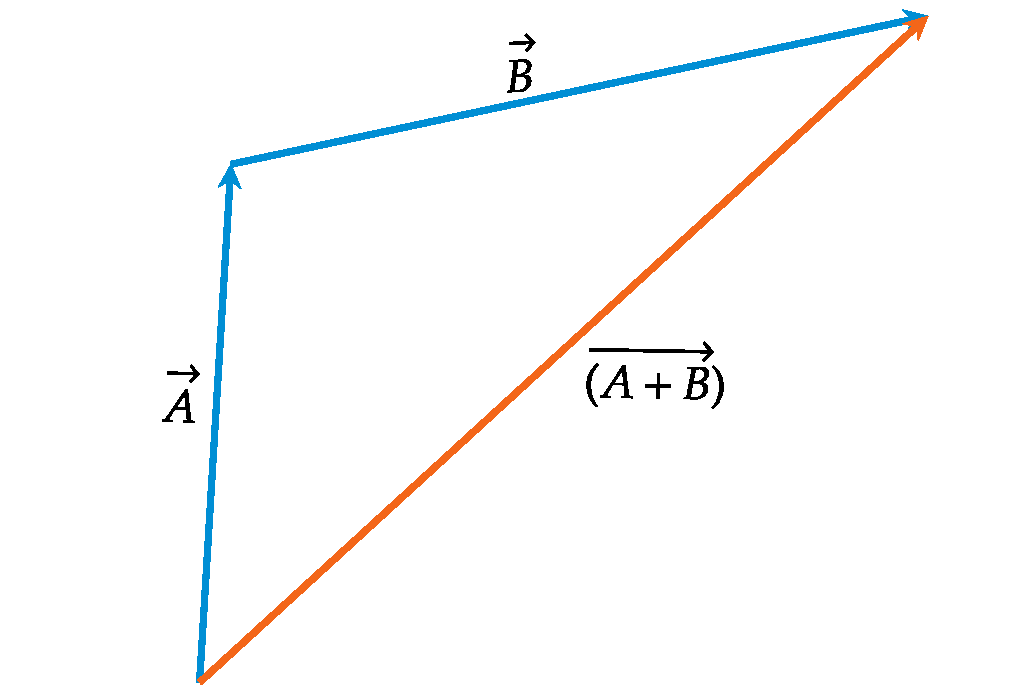
\includegraphics[width=0.70\textwidth]{Triangular}
		\caption{Triangular law of vector addition}
		\end{minipage}\hfil
	\begin{minipage}{0.45\textwidth}
	\centering
	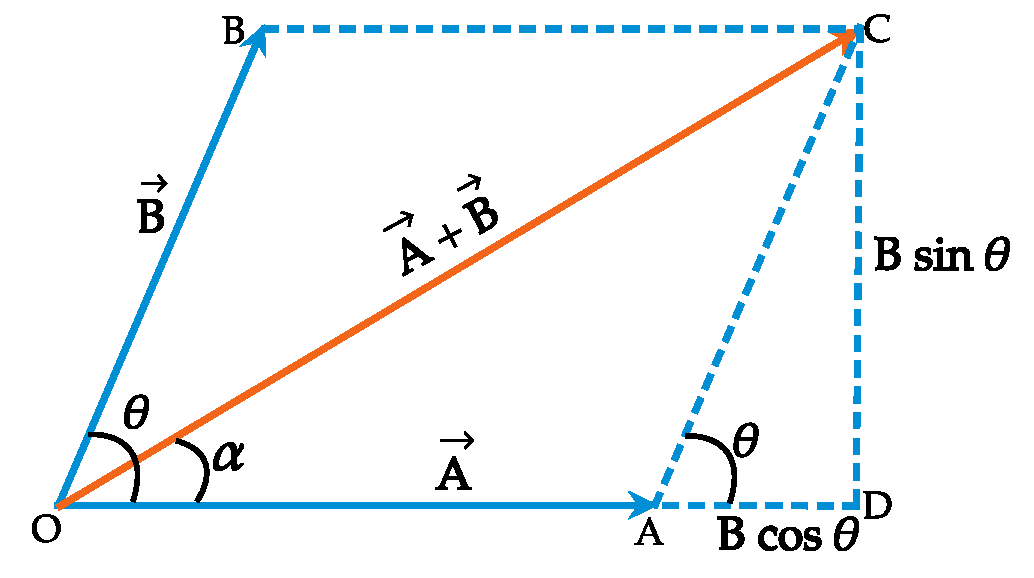
\includegraphics[width=0.75\textwidth]{parellelogram}
	\caption{Parellelogram law of vector addition}
\end{minipage}

\end{figure}

\item \textbf{Parellelogram law of vector addition:}
\\ \\When two vectors act at a point, their resultant is found by the law of parallelogram of vectors.(We got to use it often in Electricity and magnetism.)

The magnitude of Resultant vector ${\vec{A }+\vec{B}}$
From right angled $\triangle$ OCD.
\begin{align*}
O C^{2}&=O D^{2}+C D^{2}\\
&=(O A+AD)^{2}+C D^{2}\\
&=O A^{2}+A D^{2}+2AD\cdot OA +C D^{2}\\\\
\text{Here,}\hspace{1.3cm} O A&= A\ ; \ AD=B\cos\theta \ ; \ CD= B\sin\theta\\\\
\text{Then,}\hspace{1.1cm}  O C^{2}&=|\vec{A }+\vec{B}|^{2}\\&=A^{2}+(B\cos\theta)^{2}+(B\sin\theta)^{2}+2AB\cos\theta\\&=A^{2}+B^{2}+AB\cos\theta\\
|\vec{A }+\vec{B}|&=\sqrt{A^{2}+B^{2}+2AB\cos\theta}\\
\\
\text{The direction of }&\text{ Resultant vector}\ {\vec{A }+\vec{B}} \ \text{with the vector}  \ {\vec{A}}\\
\tan \alpha&=\frac{B \sin \theta}{A+B \cos \theta}\\
\alpha&=\tan ^{-1}\left(\frac{B \sin \theta}{A+B \cos \theta}\right)\\
\text{If the  two vectors}&\text{   are parellel i.e., $\theta=0$ \ Then,  }\ \\
|\vec{A }+\vec{B}|&=\sqrt{A^{2}+B^{2}+2AB}=\sqrt{(A+B)^{2}}=(A+B)\\
\text{If the  two vectors}&\text{   are anti-parellel i.e., $\theta=180$ \ Then,  }\ \\
|\vec{A }+\vec{B}|&=\sqrt{A^{2}+B^{2}-2AB}=\sqrt{(A-B)^{2}}=(A-B)\\
\end{align*}
\end{itemize}
\begin{note}
	\leavevmode
	\\\\
     	If $|\vec{A}|=|\vec{B}|=A$ Then resultant of these two vectors will be,
	\begin{enumerate}
		\item $\theta=0\qquad \rightarrow \sqrt{A^{2}+A^{2}+2A A\cos 0} \hspace{0.2cm}=\sqrt{A^{2}+A^{2}+2A^{2}}=2A $ 
		\item $\theta=60^{\circ} \quad\rightarrow \sqrt{A^{2}+A^{2}+2A A\cos 60}=\sqrt{A^{2}+A^{2}+A^{2}} =\sqrt{3}A $
		\item $\theta=90^{\circ}\quad\rightarrow \sqrt{A^{2}+A^{2}+2A A\cos 90}=\sqrt{A^{2}+A^{2}}=\sqrt{2} A $
			\item $\theta=180^{\circ} \hspace{0.3cm} \rightarrow \sqrt{A^{2}+A^{2}+2A A\cos 180}=\sqrt{A^{2}+A^{2}-2A^{2}} =0 $ 
	\end{enumerate}
\end{note}

\subsubsection{Properties of vector addition}
\begin{itemize}
	\item Commutation property:
	$\mathbf{A}+\mathbf{B}=\mathbf{B}+\mathbf{A}$.
	\item Associative property:$(\mathbf{A}+\mathbf{B})+\mathbf{C}=\mathbf{A}+(\mathbf{B}+\mathbf{C})$.
	\item Additive identity:$\mathbf{A}+\mathbf{0}=\mathbf{A} \quad$.
	\item Additive inverse:$\mathbf{A}+(-\mathbf{A})=\mathbf{0} \quad$ .
	
\end{itemize}
\subsection{Vector  multiplication}
\subsubsection{\large{1}.{Scaling of vector}(Multiplication by scalar)}
Scaling a vector means changing it's length by a scale factor.	Multiplication of a vector by a positive scalar $'c'$, multiplies the magnitude but leaves the
direction unchanged. If $'c'$ is negative, the direction is reversed.
\begin{figure}[H]
	\begin{center}
		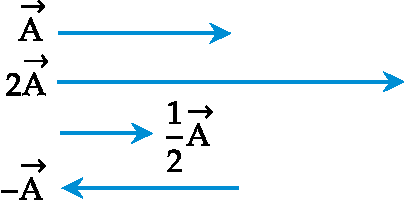
\includegraphics[width=0.30\textwidth]{scaling}
	\end{center}
\caption{Scaling of vector}
\end{figure}
\subsubsection{Properties of scalar multiplication}
\begin{itemize}
	\item  Distributive property:\quad$a(\vec{\mathrm A}+\vec{\mathrm B})=a \vec{\mathrm A}+a \vec{\mathrm B}$.
\end{itemize}
\subsubsection{\large{2}.Dot product or scalar product of two vectors}
The dot product of two vectors is defined as
\begin{equation}
$$\vec{A} \cdot \vec{B}=|A| | B| \cos \theta$$
\end{equation}
Where $\theta$ is the angle they form when placed tail to tail. $\vec{\mathrm{A}} \cdot \vec{\mathrm B}$ is itself a scalar.Geometrically $\vec{\mathrm A} \cdot \vec{\mathrm B}$ is the product of $\mathrm A$ times the projection of $\vec{\mathrm B}$ along $\vec{\mathrm A}$.
\\\newline In general,\ If \ $\vec{\mathrm A}=\mathrm A_{z} \hat{i}+\mathrm A_{y} \hat{j}+\mathrm A_{z} \hat{k}$ and $\vec{\mathrm B}=\mathrm B_{x} \hat{i}+\mathrm B_{y} \hat{j}+\mathrm B_{z} \hat{k},$\\\\ Then we can construct the scalar product of $\vec{\mathrm A}$ and $\vec{\mathrm B}$ as,
\begin{equation}
$$\vec{\mathrm A} \cdot \vec{ \mathrm B}=\mathrm A_{x} \mathrm B_{x}+\mathrm A_{y} \mathrm B_{y}+\mathrm A_{z} \mathrm B_{z}$$
\end{equation}  
\begin{example}\textbf{Workdone:}
	If a constant force $F$ acting on a particle displaces it from the point A to B then,\\
	\begin{minipage}{0.45\textwidth}
		\begin{align*}
		\text{Work done} &=\text{(component of F along A B ). Displacement}\\
		&=\mathrm{F} \cos \theta . A B \\
		&=\vec{F} \cdot \overrightarrow{A B}\\
		\text{Work done }&=\text{Force. Displacement}
		\end{align*}
	\end{minipage}
	\begin{minipage}{0.45\textwidth}
	\begin{figure}[H]
		\begin{center}
			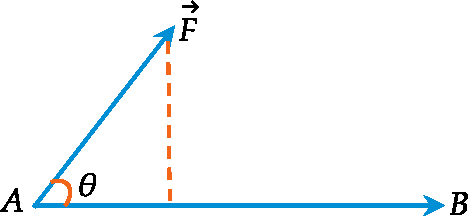
\includegraphics[width=0.65\textwidth]{workdone}
		\end{center}
		\caption{Workdone}
	\end{figure}
\end{minipage}
\end{example}
\subsubsection{Projection:}Projection of a vector A on B is the component of vector A in the direction of vector B.$$\text{Projection of}\quad \vec{\mathrm A} \text{\quad along}\quad \vec{\mathrm B} =\vec{\mathrm A}\cos\theta =\vec{\mathrm A} \cdot \hat{\mathrm B}$$.
\subsubsection{Properties of Dot product}
\begin{itemize}
	\item Commutative property:$\vec{\mathrm A} \cdot \vec{\mathrm B} =\vec{\mathrm B} \cdot \vec{\mathrm A}$.
	\item Asociative property:$ \vec{\mathrm A} \cdot(\vec{\mathrm B}+\vec{\mathrm C}) =\vec{\mathrm A} \cdot \vec{\mathrm B}+\vec{\mathrm A} \cdot \vec{\mathrm C}$.
	\item For two mutually perpendicular vectors $\vec{\mathrm A}$ and $\mathrm B, \mathrm A \cdot \vec{\mathrm B}=0$.
	\item If the two vectors are parallel, $\vec{\mathrm A} \cdot \vec{\mathrm B}=\mathrm {A B}$.(since, $\cos0=1$)
	\item $\hat{i} \cdot \hat{j}=\hat{j} \cdot \hat{k}=\hat{k} \cdot i=0\newline  \hat{i} \cdot \hat{i}=\hat{j}\cdot\hat{j} = \hat{k}\cdot \hat{k}=1$\\\\ 
\end{itemize}
\begin{exercise}
	For the two vectors  $ \vec{A}=6\hat{i}+4\hat{j}+3\hat{k}$ and $ \vec{B}=2\hat{i}-3\hat{j}-3\hat{k}$
	\newline  $$\begin{aligned}
	\vec{\mathrm A} \cdot \vec{ \mathrm B}&=\mathrm A_{x} \mathrm B_{x}+\mathrm A_{y} \mathrm B_{y}+\mathrm A_{z} \mathrm B_{z}\\
	&=12-12-9\\
	&=-9
	\end{aligned}$$
\end{exercise}
\subsubsection{{\large 3}.Vector  product or Cross product}
Cross product of two vectors $\vec{\mathrm A}$ and $\vec{\mathrm B}$  is defined as a vector that is perpendicular (orthogonal) to both $\vec{\mathrm A}$ and $\vec{\mathrm B}$, with  a magnitude equal to the area of the parallelogram that the vectors span(This suggest that area may be treated as a vector quantity). Since there are two opposite directions which are so perpendicular to $\vec{A} \ \text{and} \ \vec{B}$  This does not uniquely determine $\vec{A} \times \vec{B}$ . The direction of $\vec{A} \times \vec{B}$ is fixed by a convention, called the Right Hand Rule.\\\\
\textbf{Right Hand Rule :}\\
Stretch out the fingers of the right hand so that the thumb becomes perpendicular to both the index (fore
finger) and the middle finger. If the index points in the direction of $\vec{A}$ and the middle finger in the direction of
$\vec{B}$ then, $\vec{A} \times \vec{B}$ points in the direction of the thumb.\\\\
The vector product of $\vec{A} \ \text{and} \ \vec{B}$  is defined as, 
\begin{equation}
$$\vec{\mathrm A} \times \vec{\mathrm B}=|\vec{\mathrm A}||\vec{\mathrm B}| \sin \theta  \hat{n}$$
\end{equation}
Where $\hat{n}$ is unit vector normal to the plane containing $\vec{\mathrm A}$ and $\vec{\mathrm B}$.
\\Using decomposition of vector into their cartesian components,we can find $\vec{\mathrm A} \times \vec{\mathrm B}$ as,
\\ If $\vec{\mathrm A}=\mathrm A_{z} \hat{i}+\mathrm A_{y} \hat{j}+\mathrm A_{z} \hat{k}$ and $\vec{\mathrm B}=\mathrm B_{x} \hat{i}+\mathrm B_{y} \hat{j}+\mathrm B_{z} \hat{k},$ then $$\vec{\mathrm A} \times \vec{\mathrm B}=\left|\begin{array}{lll}\hat{i} & \hat{j} & \hat{k} \\ \mathrm A_{x} & \mathrm A_{y} & \mathrm A_{z} \\ \mathrm B_{x} & \mathrm B_{y} & B_{z}\end{array}\right|$$
\begin{example}
	Angular momentum
	\newline The angular momentum of a particle, about a reference point , is defined as the vector product of the potion relative to the reference point, and momentum of the particle
	 $$ L=r\times p$$
	 \begin{figure}[H]
	 	\begin{center}
	 		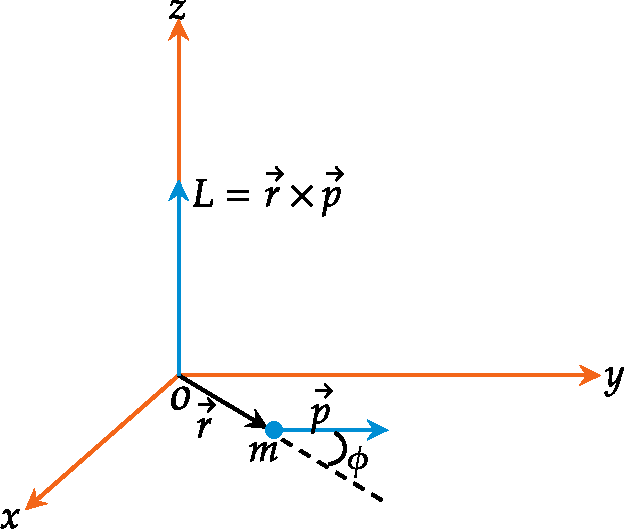
\includegraphics[width=0.30\textwidth]{angular momentum}
	 	\end{center}
 	\caption{Angular momentum}
	 \end{figure}
\end{example}
\subsubsection{Properties of Cross product} 
\begin{itemize}
	\item Distributive property\hspace{0.7cm}:\ $\vec{\mathrm A} \times(\vec{\mathrm B} + \vec{\mathrm C})=(\vec{\mathrm A} \times \vec{\mathrm B})+(\vec{\mathrm A} \times \vec{\mathrm C})$
	\item Commutative property\quad:\ $\vec{\mathrm A} \times \vec{\mathrm B}=-(\vec{\mathrm B} \times \vec{\mathrm A})$.
	\item For two collinear vectors (parallel or anti-parallel vectors) $\vec{\mathrm A} \times \vec{\mathrm B}=0$.
	\item $\hat{i} \times \hat{i}=\hat{j} \times \hat{j}=\hat{k} \times \hat{k}=0\\\\
	\; \ \hat{i} \times \hat{j}=\hat{k}
	\; \ \hat{j} \times \hat{k}=\hat{i}
	\; \ \hat{k} \times \hat{i}=\hat{j}$.
	
\end{itemize}
\begin{exercise}
	Find the area of a parallelogram whose adjacent sides are $\hat{i}-2 \hat{j}+3 \hat{k}$ and
	$2 \hat{i}+\hat{j}-4 \hat{k}$.
\end{exercise}
\begin{answer}
	\begin{align*}
\text{Vector area of parellelogram}&=\left|\begin{array}{rrr}\hat{i} & \hat{j} & \hat{k} \\ 1 & -2 & 3 \\ 2 & 1 & -4\end{array}\right|\\
&=(8-3) \hat{i}-(-4-6) \hat{j}+(1+4) \hat{k}=5 \hat{i}+10 \hat{j}+5 \hat{k}\\
\text{Area of parallelogram}&=\sqrt{(5)^{2}+(10)^{2}+(5)^{2}}=5 \sqrt{6}
\end{align*}
\end{answer}


\subsubsection{4.Triple product}
\begin{itemize}
	\item \textbf{Scalar Triple product}
	\\The scalar triple product of three vectors $\vec{\mathrm{A}}, \vec{\mathrm{B}}$, and $\vec{\mathrm{C}}$ is $(\vec{\mathrm{A}} \times\vec{\mathrm{B}}) \cdot \vec{\mathrm{C}} .$ It is a scalar product because, just like the dot product, it evaluates to a single number.  The absolute value of $|(\vec{\mathrm{A}} \times \vec{\mathrm{B}}) \cdot \vec{\mathrm{C}}|$ is the volume of the parallelepiped spanned by $\vec{\mathrm{A}}, \vec{\mathrm{B}},$ and $\vec{\mathrm{C}}$ (i.e., the parallelepiped whose adjacent sides are the vectors $\vec{\mathrm{A}}, \vec{\mathrm{B}},$ and $\vec{\mathrm{C}}$ ).\begin{figure}[H]
		\begin{center}
			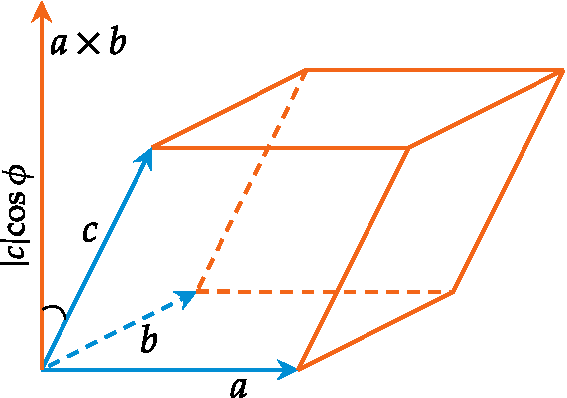
\includegraphics[width=0.25\textwidth]{parellelopiped}
		\end{center}
	\caption{Scalar triple product}
	\end{figure}
\begin{align*}
	\vec{\mathrm A} \cdot(\vec{\mathrm B} \times \vec{\mathrm C})&=\vec{\mathrm B} \cdot(\vec{\mathrm C} \times \vec{\mathrm A})=\vec{\mathrm C} \cdot(\vec{\mathrm A} \times \vec{\mathrm B})\\
	\text{In component form}\ \vec{\mathrm A} \cdot(\vec{\mathrm B} \times \vec{\mathrm C})&=\left|\begin{array}{lll}\mathrm A_{x} & \mathrm A_{y} & \mathrm A_{z} \\ \mathrm B_{x} & \mathrm B_{y} & \mathrm B_{z} \\ \mathrm C_{x} & \mathrm C_{y} & \mathrm C_{z}\end{array}\right|\\
\end{align*}

	\item \textbf{Vector Triple product}
	\\A vector triple product $\vec{\mathrm A} \times(\vec{\mathrm B} \times \vec{\mathrm C})$ of 3 vectors ,$\vec{\mathrm A}$ , $\vec{\mathrm B}$ and $\vec{\mathrm C}$ is simply a vector lying in the plane containing $\vec{\mathrm A}$ , $\vec{\mathrm B}$ and $\vec{\mathrm C}$.\\

	The vector triple product can be simplified by the so-called $\text{ B A C}-\text{ C A B}$ rule.The equation is linear in  A,B and C.
	$$
	\vec{\mathrm A} \times(\vec{\mathrm B} \times \vec{\mathrm C})=\vec{\mathrm B}(\vec{\mathrm A} \cdot \vec{\mathrm C})-\vec{\mathrm C}(\vec{\mathrm A} \cdot \vec{\mathrm B})
	$$
\end{itemize}
\begin{note}

Suppose we have two vectors $ \vec{a}$ and $ \vec {b}$ as shown in the figure.
\ref{vector}
We can write $\vec{b}$ as
$$\vec{b}=\vec{{b_{\parallel}}}+\vec{{b_{\perp}}} $$
Where ${b_{\parallel}}$ is the projection of $ \vec {b}$ along  $ \vec{a}$ and$ \vec{{b_{\perp}}}$ is the projection of  $ \vec {b}$ perpendicular to $ \vec{a}$\\
\begin{minipage}{0.65\textwidth}
	\begin{align*}
	\vec {b}=&(\vec{b}\cdot \hat{a})\cdot \hat{a}+\vec{{b_{\perp}}}\\
	\vec {b}=&\frac{(\vec{b}\cdot \vec{a})\cdot\vec{a}}{a^{2}}+\vec{{b_{\perp}}}\\
	\vec {b}=&\frac{(\vec{b}\cdot \vec{a})\cdot\vec{a}}{a^{2}}+{\vec{b}-\frac{(\vec{b}\cdot \vec{a})\cdot\vec{a}}{a^{2}}}\\
	\vec {b}=&\frac{(\vec{b}\cdot \vec{a})\cdot\vec{a}}{a^{2}}+\frac{\vec{b}(\vec{a}\cdot\vec{a})-{(\vec{b}\cdot\vec{a})\vec{a}}}{a^{2}}\\
	\vec {b}=&\frac{(\vec{b}\cdot \vec{a})\cdot\vec{a}}{a^{2}}+\frac{\vec{a}\times(\vec{b}\times\vec{a})}{a^{2}}\\
	\vec{b}=&\vec{{b_{\parallel}}}(\text{parellell component})+\vec{{b_{\perp}}}(\text{perpendicular component})
	\end{align*}
\end{minipage}
\begin{minipage}{0.35\textwidth}\hfill
\begin{figure}[H]
	\begin{center}
		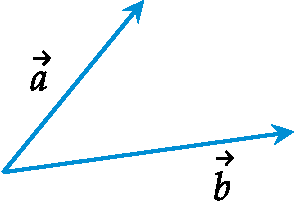
\includegraphics[width=0.8\textwidth]{vector1}
	\end{center}
\caption{vector}
\label{vector}
\end{figure}
\end{minipage}
\end{note}

\section{General curvilinear coordinate system}\index{General culvilinear coordinate system}
Not all Physical problems  are well adapted to a solution in cartesian coordinate system.We have to develop a general system that may be apt for any particular system of intersect.
The coordinates in general curvilinear coordinate system be described by three coordinates, $q_{1},q_{2} $ and $ q_{3}$\\then  a position vector $ \vec{ r}$ in the system can be represented as,
\begin{align*}
\vec{r}&=\vec{r}(q_{1},q_{2},q_{3})\\
\text{Then,}\quad
 dr&={\frac{\partial r}{\partial q_{1} }} dq_{1}+{\frac{\partial r}{\partial q_{2} }} dq_{2}+{\frac{\partial r}{\partial q_{3} }} dq_{3}
\end{align*}
Where,\ ${\frac{\partial r}{\partial q_{1} }}$,${\frac{\partial r}{\partial q_{2} }}$,${\frac{\partial r}{\partial q_{3} }}$ are the tangent vectors along $q_{1},q_{2}  $ and \ $q_{3}$.
\\\\The unit vectors along $q_{1},q_{2}  $ and \ $q_{3}$ are defined as,
$$ \hat e_{1}=\frac{{\frac{\partial r}{\partial q_{1} }}}{|{\frac{\partial r}{\partial q_{1} }}|}\quad ;\quad
 \hat e_{2}=\frac{{\frac{\partial r}{\partial q_{2} }}}{|{\frac{\partial r}{\partial q_{2} }}|}\quad ;\quad\hat e_{3}=\frac{{\frac{\partial r}{\partial q_{3} }}}{|{\frac{\partial r}{\partial q_{3} }}|}$$
\\
\textbf{Scaling factor:}\\\\
The factor ${|{\frac{\partial r}{\partial q_{1} }}|}$ is known as the scaling factor. It is denoted as $h_{1}$.\\\\
Similiarly, $h_{2}={|{\frac{\partial r}{\partial q_{2} }}|}$
and $h_{3}={|{\frac{\partial r}{\partial q_{3} }}|}$\\
\\Then the position vector can be written as,
\begin{equation}
$$ \vec dr=h_{1}\hat e_{1} dq_{1}+h_{2}\hat e_{2} q_{2}+h_{3}\hat e_{3}q_{3}$$
\end{equation}
\textbf{Cartesian coordinate system}
\begin{alignat*}{4}
&\text{Coordinates}&& \textbf{:} \ q_{1}=x\;\ q_{2}=y\;\ q_{3}=z\\
&\text{Scaling factors} && \textbf{:}\ h_{1}=1\; \ h_{2}=1\;\  h_{3}=1\\
&\text{Unit vectors}&&\textbf{:}\ \hat{e}_{1}=\hat{e}_{x}\;\ \hat{e}_{2}=\hat{e}_{y}\;\ \hat{e}_{3}=\hat{e}_{z}\\
&\text{Position vector}&&\textbf{:} \ \vec dr=\hat e_{x} dx+\hat e_{y} dy+\hat e_{z}dz
\end{alignat*}

\section{Differential Operations on Vectors}\index{Differential Operations on Vectors}
\begin{alignat*}{2}
&\text{Gradient }(\nabla)&&\textbf{:}\ \text{A derivative on a scalar that gives a vector.}
\\&\text{Curl} (\nabla \times)&&\textbf{:}\ \text{A derivative on a vector that gives another vector.}
\\&\text{Divergence }(\nabla \cdot)&&\textbf{:}\ \text{A derivative on a vector that gives scalar.}
\end{alignat*}
 
\subsection{Gradient}
 The gradient is the multidimensional rate of change of a particular function.
Gradient of a continuously differentiable scalar function $\phi(q_{1}, q_{2}, q_{3})$ is mathematically defined as:
$$ \nabla \phi=\frac{1}{h_{1}}\frac{\partial \phi}{\partial q_{1}} \hat e_{1}+\frac{1}{h_{2}}\frac{\partial \phi}{\partial q_{2}} d \hat e_{2}+\frac{1}{h_{3}}\frac{\partial \phi}{\partial q_{3}} \hat e_{3}
$$
\subsubsection{Physical interpretation}
	Gradient tells you how much something changes as you move from one point to another (such as the pressure in a stream). If a surface $\phi(x, y, z)=c$ passes through a point $P$. The value of the function at each point on the surface is the same as at $P$. Then such a surface is called a level surface through $P$. At each point of the level surafce, the value of scalar function $f$ will be same. Equipotential surface on which value of electrostatic potential is same at all points.


	\begin{figure}[H]
		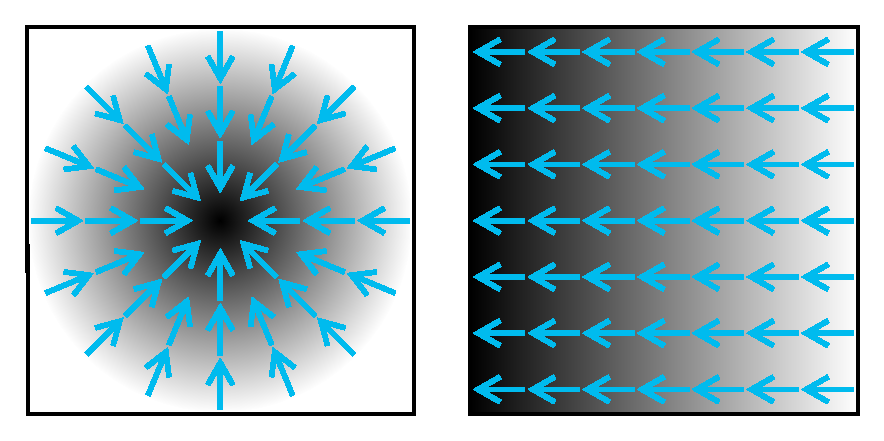
\includegraphics[width=.85\textwidth]{Gradient2}
		\caption{The gradient, represented by the blue arrows, denote the direction of greatest change of a scalar function. The values of the function are represented in greyscale and increase in value from white (low) to dark (high).}
	\end{figure}




\subsubsection{Product rule}$ \bullet$ $\vec{\nabla}(\phi \psi)=\phi \vec{\nabla} \psi+\psi \vec{\nabla} \phi$
\\$ \bullet$ $\vec{\nabla}(\overrightarrow{\mathrm{A}} \cdot \overrightarrow{\mathrm{B}})=\overrightarrow{\mathrm{A}} \times(\vec{\nabla} \times \overrightarrow{\mathrm{B}})+\overrightarrow{\mathrm{B}} \times(\vec{\nabla} \times \overrightarrow{\mathrm{A}})+(\overrightarrow{\mathrm{A}} \cdot \vec{\nabla}) \overrightarrow{\mathrm{B}}+(\overrightarrow{\mathrm{B}} \cdot \vec{\nabla}) \overrightarrow{\mathrm{A}}$
\\
\\\textbf{Normal and Directional derivative}
 \\\\\textbf{ Normal:}\newline If $\phi(x, y, z)=c$,  represents a family of surfaces for different values of the constant
 c. On differentiating $\phi,$ 

\begin{align*}
	 \text{We get,} \hspace{0.8cm}  d \phi&=0
	\\\text{But,} \hspace{0.8cm} d \phi&=\nabla \phi \cdot d \vec{r} \quad \\
	\text{So,} \hspace{0.05cm} \quad \nabla \phi \cdot d r&=0
	\end{align*}
The scalar product of two vectors $\nabla \phi$ and $d \vec{r}$ being zero, $\nabla \phi$ and $d \vec{r}$ are perpendicular to each other. Then, $d \vec{r}$ is in the direction of tangent to the given surface.

	\begin{itemize}
	\item  Normal vector to the level surface\hspace{1.2cm}: $\vec{\nabla} \phi$ 
	\item   Unit normal vector to the level surface\quad: $\hat{n}=\frac{\vec{\nabla} \phi}{|\vec{\nabla} \phi|}$
\end{itemize}
	
\begin{exercise}
	 Find the unit normal to the surface:$x^{2}+y^{2}=z$ at a point (1,2,5) \end{exercise}
	 \begin{answer}
	 		\begin{align*}
	 		\text{Let}\ \phi&=x^{2}+y^{2}-z\\
	 		\nabla \phi&=\left(\hat{i} \frac{\partial}{\partial x}+\hat{j} \frac{\partial}{\partial y}+\hat{k} \frac{\partial}{\partial z}\right)\left(x^{2}+y^{2}-z\right)=2 x \hat{i}+2 y \hat{j}-\hat{k}\\
	 		(\nabla \phi)_{1,2,5}&=2 \hat{i}+4 \hat{j}-\hat{k}\\
	 		\text { Unit normal vector }&=\frac{\Delta \phi}{|\Delta \phi|}\\&=\frac{2 \hat{i}+4 \hat{j}-\hat{k}}{\sqrt{4+16+1}}\\&=\frac{2}{\sqrt{21}} \hat{i}+\frac{4}{\sqrt{21}} \hat{j}-\frac{\hat{k}}{\sqrt{21}}
	 	\end{align*}
	 \end{answer}

	
 \subsubsection{Directional derivative} Directional derivative of $\phi$ in the direction of $\vec{A}$ is defined as rate of change of
$\phi$ with distance along the direction of $\vec{A}$. It is mathematically defined as the component of $\vec{\nabla} \phi$ in the direction of vector $\vec{A}$ i.e.
\begin{equation*}
 \vec{\nabla} \phi\cdot{{\hat A}}=\vec{\nabla} \phi.\frac{\vec A}{|\vec{A}|}
\end{equation*}
\begin{exercise}
	Find the directional derivative of $\phi(x, y, z)=x^{2} y z+4 x z^{2}$ at (1,-2,1) in the direction of $2 \hat{i}-\hat{j}-2 \hat{k}$.\end{exercise}
\begin{answer}
		\begin{align*}
		\phi(x, y, z)&=x^{2} y z+4 x z^{2}\\
		\nabla \phi&=\left(\hat{i} \frac{\partial}{\partial x}+\hat{j} \frac{\partial}{\partial y}+\hat{k} \frac{\partial}{\partial z}\right)\left(x^{2} y z+4 x z^{2}\right)\\
		&=\left(2 x y z+4 z^{2}\right) \hat{i}+\left(x^{2} z\right) \hat{j}+\left(x^{2} y+8 x z\right) \hat{k} \\
		\nabla \phi \text { at }(1,-2,1) &=\left\{2(1)(-2)(1)+4(1)^{2}\right\} \hat{i}+(1 \times 1) \hat{j}+\{1(-2)+8(1)(1)\} \hat{k} \\
		&=(-4+4) \hat{i}+\hat{j}+(-2+8) \hat{k}=\hat{j}+6 \hat{k} \\
		\hat{a} &=\text { unit vector }=\frac{2 \hat{i}-\hat{j}-2 \hat{k}}{\sqrt{4+1+4}}=\frac{1}{3}(2 \hat{i}-\hat{j}-2 \hat{k})
		\intertext{So, the  directional derivative at (1,-2,1)}&=\nabla \phi \cdot \hat{a}\\
		&=(\hat{j}+6 \hat{k}) \cdot \frac{1}{3}(2 \hat{i}-\hat{j}-2 \hat{k})\\&=\frac{1}{3}(-1-12)=\frac{-13}{3}
	\end{align*}
\end{answer} 
\subsubsection{Tangent planes}
\vspace{-0.8cm}
\begin{minipage}{0.6\textwidth}
	Consider $\phi(x, y, z)=c$ be the equation of a level surface, and $\vec{r}=x_{0} i+y_{0}\hat{j}+z_{0} \hat{k}$ be the position vector of
any point $\mathrm{P}(x, y, z)$ on this surface. \\\\Since, $ \vec{\nabla} \phi$ is a vector normal to the surface, it is perpendicular to the tangent plane at
P. 
\end{minipage}
\begin{minipage}{0.4\textwidth}
	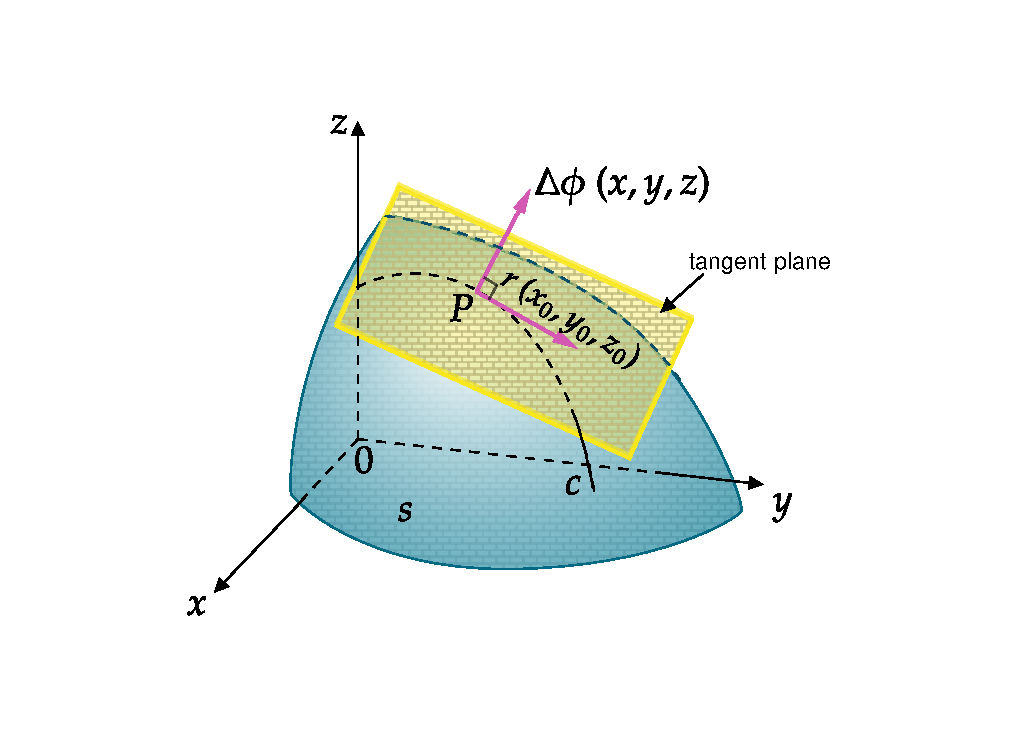
\includegraphics[width=8cm]{tangent plane}
\end{minipage}


 Let, $\vec{R}=x\hat{i}+y \hat{j}+z\hat{k}$ be the position vector of any point on the tangent plane at $P$ to the surface.\\\\  Then,
$\vec{R}-\vec{r}=(x-x_{0}) \hat{i}+(y-y_{0}) \hat{i}+(z-z_{0}) \hat{k}$ lies in the tangent plane at $P$ and it will be perpendicular to $\vec{\nabla} \phi$
\\Then the tangent plane at the point P :\begin{align*}
(\vec{R}-\vec{r}) \cdot \vec{\nabla} \phi&=0\\
(x-x_{0}) \frac{\partial \phi}{\partial x}+(y-y_{0}) \frac{\partial \phi}{\partial y}+(z-z_{0}) \frac{\partial \phi}{\partial z}&=0
\end{align*}

 


%...........................................................................................
\subsection{Divergence ($\nabla \cdot$)}
The divergence of a vector field measures how much the flow is expanding at a given point. It does not indicate in which direction the expansion is occuring. Hence the divergence is a scalar. Divergence of a continuous differentiable vector point function $A$ specified in a vector field is given
by,
$$
{\nabla} \cdot \vec{f}=\frac{1}{h_{1} h_{2} h_{3}}\left[\frac{\partial}{\partial q_{1}}\left(h_{2} h_{3} f_{1}\right)+\frac{\partial}{\partial q_{2}}\left(h_{3} h_{1} f_{2}\right)+\frac{\partial}{\partial q_{3}}\left(h_{1} h_{2} f_{3}\right)\right]
$$
In Cartesian coordinate system,

$$ \nabla.f=\frac{\partial f_{1}}{\partial x}+\frac{\partial f_{2}}{\partial y}+\frac{\partial f_{3}}{\partial z}$$
You can't
have the divergence of a scalar: that’s meaningless.


\subsubsection{Physical interpretation}
$\vec{\nabla} \cdot \vec{A}$ is a measure of how much the vector $\vec{A}$ spreads out (diverges) from a point in space.
\begin{figure}[H]
	\begin{center}
		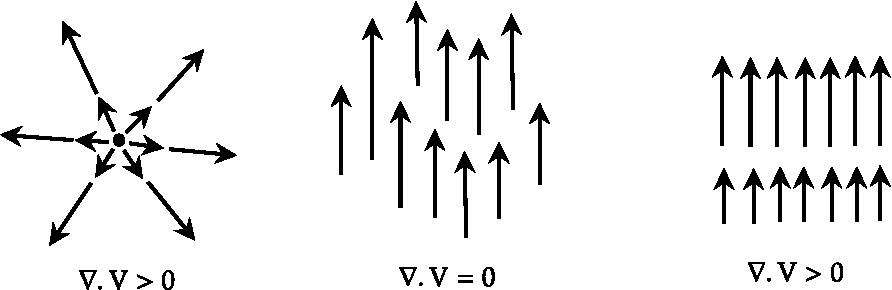
\includegraphics[width=9cm,height=3cm]{divergence-crop}
	\end{center}
\caption{Physical intepretation of divergence.}
\end{figure}

\begin{note}
	$\bullet$ If $\vec{\nabla} \cdot \vec{A}=0,$ then $\vec{A}$ is known as solenoidal vector field.
	\\$\bullet$ If $\vec{\nabla} \cdot \vec{A}=$ negative, then $\vec{A}$ is known as sink field i.e. vector lines are going inward.
	\\$\bullet$ If $\vec{\nabla} \cdot \vec{A}=$ positive, then $\vec{A}$ is known as source field i.e. vector lines are the going outward.
\end{note}
\textbf{Product rules}\\\\$\bullet$ $\vec{\nabla} \cdot(f \overrightarrow{\mathrm{A}})=f(\vec{\nabla} \cdot \overrightarrow{\mathrm{A}})+\overrightarrow{\mathrm{A}} \cdot(\vec{\nabla} f)$
$\\\bullet \vec{\nabla} \cdot(\vec{A} \times \vec{B})=\vec{B} \cdot(\vec{\nabla} \times \vec{A})-\vec{A} \cdot(\vec{\nabla} \times \vec{B})$
\begin{exercise}
	 
	Calculate $\nabla \cdot \vec{ r}$\end{exercise}
	 \begin{answer}
	 
	 \begin{align*}
	 	\vec{ r}&=x\hat{i}+y\hat{j}+z\hat{k}\\
	 	\nabla \cdot \vec{ r} &=\left(\hat{i} \frac{\partial}{\partial x}+\hat{j} \frac{\partial}{\partial y}+\hat{k} \frac{\partial}{\partial z}\right) \cdot (x\hat{i}+y\hat{j}+z\hat{k})\\
	 	&=\frac{\partial x}{\partial x}+\frac{\partial y}{\partial y}+\frac{\partial z}{\partial z}\\
	 	&=1+1+1\\
	 	&=3
	 \end{align*}
	 
	 
	 \end{answer}
	 
	 

\subsection{Curl}
The curl is the vector valued derivative of a vector function. Its operation can be geometrically interpreted as the rotation of a field about a point in space.\\From the definition of $\vec{\nabla}$ we construct the curl of a vector $\vec{f}=f_1\hat{e}_{1}+f_2\hat{e}_{2}+f_3\hat{e}_{3}$ as
$$
\nabla \times \vec{f
}=\frac{1}{h_{1} h_{2} h_{3}}\left|\begin{array}{lll}
	h_{1} \hat{e}_{1} & h_{2} \hat{e}_{2} & h_{3} \hat{e}_{3} \\
	\partial / \partial q_{1} & \partial / \partial q_{2} & \partial / \partial q_{3} \\
	h_{1} f_{1} & h_{2} f_{2} & h_{3} f_{3}
\end{array}\right|
$$
In cartesian coordinate system,
$$
\nabla \times \vec{f
}=\left|\begin{array}{lll}
\hat{{i}} & \hat{{j}} & \hat{{k}} \\
\partial / \partial x & \partial / \partial y & \partial / \partial z \\
f_{1} & f_{2} & f _{3}
\end{array}\right|
$$

%...........................................................................................
\subsubsection{Physical interpretation}
\begin{figure}[H]
	\begin{center}
		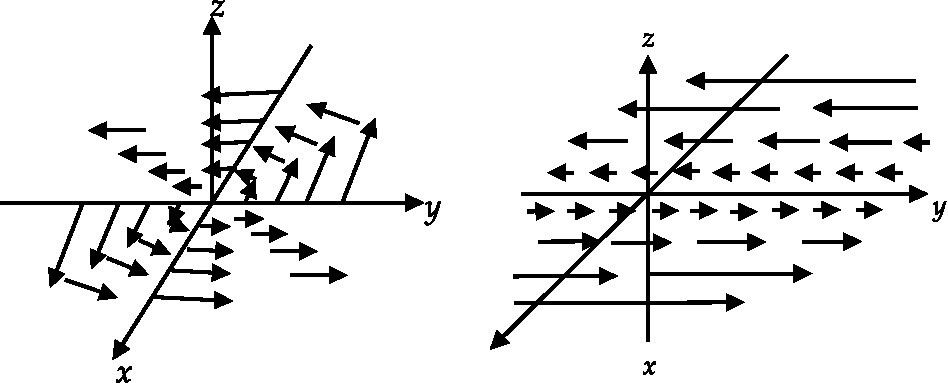
\includegraphics[width=9cm,height=4cm]{coordinate2}
	\end{center}
	\caption{Physical interpretation of Curl}
\end{figure}
The curl of a vector field measures the tendency for the vector field to swirl around. Imagine that the vector field represents the velocity vectors of water in a lake. If the vector field swirls around, then when we stick a paddle wheel into the water, it will tend to spin. The amount of the spin will depend on how we orient the paddle. Thus, we should expect the curl to be vector valued.\\
\\$\bullet \ $ If $\vec{\nabla} \times \vec{V}=0,$ then $\vec{V}$ is known as an irrotational vector and we can write $\vec{V}=\vec{\nabla} \phi$
\\$\bullet \ $ If $\vec{\nabla} \times \vec{V} \neq 0,$ then $\vec{V}$ is known as rotational vector.
\\\\\textbf{Product rules}\\
\\$\bullet \ \vec{\nabla} \times(f \overrightarrow{\mathrm{A}})=f(\vec{\nabla} \times \overrightarrow{\mathrm{A}})-\overrightarrow{\mathrm{A}} \times(\vec{\nabla} f)$
$\\\bullet \ \vec{\nabla} \times(\overrightarrow{\mathrm{A}} \times \overrightarrow{\mathrm{B}})=(\overrightarrow{\mathrm{B}} \cdot \vec{\nabla} ) \overrightarrow{\mathrm{A}}-(\overrightarrow{\mathrm{A}} \cdot \vec{\nabla}) \overrightarrow{\mathrm{B}}+\overrightarrow{\mathrm{A}}(\vec{\nabla} \cdot \overrightarrow{\mathrm{B}})-\overrightarrow{\mathrm{B}}(\vec{\nabla} \cdot \overrightarrow{\mathrm{A}})$

\begin{exercise}
	 Prove that $\left(y^{2}-z^{2}+3 y z-2 x\right) \hat{i}+(3 x z+2 x y) \hat{j}+(3 x y-2 x z+2 z) \hat{k}$ is  irrotational.\end{exercise}
	\begin{answer}
		For irrotational, we have to prove Curl $\bar{F}=0$.
		\begin{align*}
		\operatorname{Curl} \vec{F}&=\left|  \begin{array}{lll}
		\hat{i} & \hat{j} & \hat{k} \\
		\frac{\partial}{\partial x} & \frac{\partial}{\partial y} & \frac{\partial}{\partial z} \\
		y^{2}-z^{2}+3 y z-2 x & 3 x z+2 x y & 3 x y-2 x z+2 z
		\end{array}\right| \\
			&=(3 x-3 x) \hat{i}-(-2 z+3 y-3 y+2 z) \hat{j}+ 
		(3 z+2 y-2 y-3 z) \hat{k}\\&=0 \hat{i}+0 \hat{j}+0 \hat{k}=0
			\intertext{Thus, $\vec{F}$ is irrotational.}
		\end{align*}
		\end{answer}
	\begin{note}
		\begin{enumerate}
			\item The divergence of a curl of a vector field vanishes.
			\\$ \nabla \cdot(\nabla \times u)=0$\\If $ \nabla \cdot v=0 \Longrightarrow v= \nabla \times u$
			\item The curl of gradient of a scalar field vanishes.
			\\$ \nabla \times(\nabla \phi)=0$\\If $ \nabla \times \psi=0 \Longrightarrow \psi= \nabla  u$
		\end{enumerate}
	\end{note} 


\subsection{Laplacian}

The divergence of the gradient of a scalar function is called the Laplacian. In general culvilinear coordinate system laplacian can be written as,
\begin{align*}
\nabla^{2}=\frac{1}{h_{1} h_{2} h_{3}}\left[\frac{\partial}{\partial u_{1}}\left(\frac{h_{2} h_{3}}{h_{1}} \frac{\partial}{\partial u_{1}}\right)+\right. 
\left. \frac{\partial}{\partial u_{2}}\left(\frac{h_{1} h_{3}}{h_{2}} \frac{\partial}{\partial u_{2}}\right)+\frac{\partial}{\partial_{u_{3}}}\left(\frac{h_{1} h_{2}}{h_{3}} \frac{\partial}{\partial_{u_{3}}}\right)\right]
\end{align*}

In cartesian coordinate sytem,
$$ \nabla^{2}=\frac{\partial^{2}}{\partial x^{2}}+\frac{\partial^{2}}{\partial y^{2}}+\frac{\partial^{2}}{\partial z^{2}}$$
\begin{table}[h]
	\overfullrule=0pt
	\begin{tabular}{|p{1.8cm}|p{6cm}|p{8.5cm}|}
		\hline
		
		&\textbf{Cylindrical polar}($ \rho,\phi,z$) & \textbf{Spherical polar}(r,$\theta$,$\phi$)  \\\hline
		Scale factor&  ${\begin{array}{l}
				h_{1}=1  \\
				h_{2}=r \\
				h_{3}=1
		\end{array}}$ &${\begin{array}{l}
				h_{1}=1  \\
				h_{2}=r \\
				h_{3}=r \sin \theta
		\end{array}}$   \\\hline
		Gradient& $$
		\frac{\partial {f}}{\partial \boldsymbol{\rho}} \hat{\rho}+\frac{1}{\rho}\frac{\partial {f}}{\partial {\phi}} \hat{\phi}+\frac{\partial {f}}{\partial {z}} \hat{{z}}
		$$\vspace{1cm}&$$
		\hat{{r}} \frac{\partial f}{\partial r}+\hat{\boldsymbol{\theta}} \frac{1}{r} \frac{\partial f}{\partial \theta}+\hat{{\phi}} \frac{1}{r \sin \theta} \frac{\partial f}{\partial \phi}
		$$\\\hline
		Divergence\vspace{1cm}& $$
		\frac{1}{\rho} \frac{\partial }{\partial \rho}\left(\rho F_{\rho}\right)+\frac{1}{\rho} \frac{\partial }{\partial \phi}\left(F_{\phi}\right)+\frac{\partial }{\partial z}\left(F_{z}\right)
		$$ & $$
		\frac{1}{\mathrm{r}^{2}} \frac{\partial}{\partial \mathrm{r}}\left(r^{2} F_{\mathrm{r}}\right)+\frac{1}{\mathrm{rsin} \theta} \frac{\partial}{\partial \theta}\left(F_{\theta} \sin \theta\right)+\frac{1}{r \sin \theta} \frac{\partial \mathrm{F}_{\phi}}{\partial \phi}
		$$ \\\hline
		Curl\vspace{1cm}&$$
		\frac{1}{\rho } \left|\begin{array}{ccc}
			\hat{\rho} & \hat{\phi} & \hat{{z}} \\
			\frac{\partial}{\partial \boldsymbol{\rho}} & \frac{\partial}{\partial \phi} & \frac{\partial}{\partial \mathbf{z}} \\
			{F}_{\rho} & {F}_{\phi} & {F}_{{z}}
		\end{array}\right|
		$$ &$$
		\frac{1}{r^{2} \sin \theta}\left|\begin{array}{ccc}
			\hat{e}_{r} & r \hat{e}_{\theta} & r \sin \theta \hat{e}_{\phi} \\
			\partial / \partial r & \partial / \partial \theta & \partial / \partial \phi \\
			F_{r} & r F_{\theta} & r \sin \theta F_{\phi}
		\end{array}\right|
		$$ \\\hline
	Laplacian	& $$\frac{\partial^{2} f}{\partial r^{2}}+\frac{1}{r} \frac{\partial f}{\partial r}+\frac{1}{r^{2}} \frac{\partial^{2} f}{\partial \theta^{2}}+\frac{\partial^{2} f}{\partial z^{2}}$$ &$$
	\frac{1}{\mathrm{r}^{2}} \frac{\partial}{\partial \mathrm{r}}\left(r^{2} \frac{\partial f}{\partial r}\right)+\frac{1}{\mathrm{r^{2}sin} \theta} \frac{\partial}{\partial \theta}\left( \sin \theta \frac{\partial f}{\partial \theta}\right)+\frac{1}{r^{2} \sin^{2} \theta} \frac{\partial^{2} f}{\partial \phi^{2}}
	$$ 
	\\\hline

	\end{tabular}
\label{differential operators}
\caption{Differential operators in general culvilinear coordinate system}
\end{table}
\vspace{1cm}
	



\subsection{Important identities}
\begin{enumerate}
	 
	\item $\nabla \cdot \nabla \vec{A}=\nabla^{2} A=\frac{\partial^{2} \vec{A}}{\partial x^{2}}+\frac{\partial^{2} \vec{A}}{\partial y^{2}}+\frac{\partial^{2} \vec{A}}{\partial z^{2}}$( The Laplace operator.)
\item $\nabla \times \nabla \vec{A}=0$
\item $\nabla \cdot \nabla \times \vec{A}=0$
	\item $\nabla \times(\nabla \times \vec{A})=\nabla(\nabla \cdot \vec{A}) \times \nabla^{2} \vec{A}$
	\item $\nabla(\nabla \cdot \vec{A})=\nabla \times(\nabla \times \vec{A})+\nabla^{2} \vec{A}$
	\item $\nabla(\vec{A}+\vec{B})=\nabla \cdot \vec{A}+\nabla \cdot \vec{B}$
\item $\nabla \times(\vec{A}+\vec{B})=\nabla \times \vec{A}+\nabla \times \vec{B}$
\item $\nabla \cdot(\vec{A} \times \vec{B})=\vec{B} \cdot(\nabla \times \vec{A})-\vec{A} \cdot(\nabla \times \vec{B})$
\item $\nabla \times(\vec{A} \times \vec{B})=(B \cdot \nabla) A-B(\nabla \cdot A)-(A \nabla)$
$\quad B+A(\nabla B)$
\end{enumerate}
\section{Integral Calculus}
\subsection{Line integration of vectors}
\begin{figure}[H]
	\begin{center}
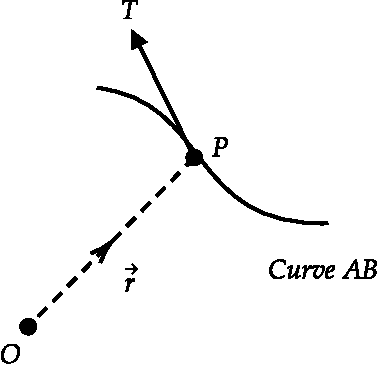
\includegraphics[width=3cm,height=3cm]{cs-01-crop}
		
	\end{center}
\caption{Line integration}
\label{line integration}	
\end{figure}
The integration of a vector function $\vec F$ along a curve is known as line integration of vectors.Infact the line integral along the curve is the integral of $\vec F$ along the tangent to the curve. 
 Consider a pont P in the curve in figure \ref{line integration} such that the position vector of P is given by $\vec r$.\\The component of $\vec F$ along the tangent at P = $\left(\vec{F} \cdot \frac{d \vec{r}}{d s}\right)$ \newline Then the Line integral of $\vec{F}$ from $A$ to $B$ along the curve $C$ will be, 
 $$\text{ Line integral}=\int_{c}\left(\vec{F} \cdot \frac{d \vec{r}}{d s}\right) d s=\int_{c} \vec{F} \cdot d \vec{r}$$


\begin{note}
	\begin{itemize}
		\item If $\vec{F}$ represents the variable force acting on a particle along arc $\mathrm{AB}$, then the total work done
		$W_{A B}=\int_{A}^{B} \vec{F} \cdot d \vec{r}$ 
		\item  If $\vec{V}$ represents the velocity of a liquid then $\oint_{c} \vec{V} \cdot d \vec{r}$ is called the circulation of $\vec{V}$ round closed curve
		$C$
		\item When the path of integration is a closed curve then notation of integration is $\oint$ in place of $\int$.
	\end{itemize}
\end{note}
\begin{example}
\textbf{Workdone}
\\  Work done by a conservative field $\vec{A}$ in moving a particle from point $P$ to $Q$ will be
$$
\int_{P}^{Q} \vec{F} \cdot \overrightarrow{d r}=\int_{P}^{Q} \vec{\nabla} \phi \cdot \overrightarrow{d r}=\int_{P}^{Q} d \phi=\phi_{Q}-\phi_{P}=\text { independent of path. }
$$
\\ Ordinarily, the value of a line integral depends critically on the particular path taken from
$a$ to $b$, but there is an important special class of vector functions for which the line
integral is independent of the path, and is determined entirely by the end points $($ A force
that has this property is called conservative).\\$\vec{A}$ in moving a particle around a closed path $C$ is $\oint_{c} \vec{F} \cdot \overrightarrow{d r}=0$
\end{example}
\begin{exercise}
	 If a force $\vec{F}=2 x^{2} y \hat{i}+3 x y \hat{j}$ displaces a particle in the xy-plane from (0,0) to
	(1,4) along a curve $y=4 x^{2} .$ Find the work done.\end{exercise}
	\begin{answer}
		\begin{align*}
		\text{Work done}&=\int_{c} \vec{F} \cdot \overrightarrow{d r} \\
		&=\int_{c}\left(2 x^{2} y \hat{i}+3 x y \hat{j}\right) \cdot(d x \hat{i}+d y \hat{j}) \\
		&=\int_{c}\left(2 x^{2} y d x+3 x y d y\right)\\
		&\left[\begin{array}{l}
		\vec{r}=x \hat{i}+y \hat{j} \\
		\overrightarrow{d r}=d x \hat{i}+d y \hat{j}
		\end{array}\right]
		\intertext{Putting the values of $y$ and $d y$, we get}
		&=\int_{0}^{1} \cdot\left[2 x^{2}\left(4 x^{2}\right) d x+3 x\left(4 x^{2}\right) 8 x d x\right]	\quad\left[\begin{array}{l}
		y=4 x^{2} \\
		d y=8 x d x
		\end{array}\right] \\
		&=104 \int_{0}^{1} x^{4} d x=104\left(\frac{x^{5}}{5}\right)_{0}^{1}=\frac{104}{5}
		\end{align*}
	\end{answer}
	



\subsection{Surface integration of vectors}

It's the two dimensional analog of line integral. Physically, it can be thought of as flow of a fluid through a surface. It is 
the integration of a vector on an open or closed surface.\\
For a function $F(x,y,z)$ the surface integral over a surface S is given as,$$S=\iint_{S}(\mathbf{F} \cdot \hat{n}) d S=\iint_{S} \mathbf{F} \cdot d \mathbf{S}$$
\\
 where $n$ is the unit normal vector to an element $d s$ and
$$
\hat{n}=\frac{\operatorname{grad} f}{|\operatorname{grad} f|} \quad d s=\frac{d x d y}{(\hat{n} \cdot \hat{k})}
$$
\begin{note}
If $\iint_{S}(\vec{F} \cdot \hat{n}) d s=0,$ then $\vec{F}$ is said to be a solenoidal vector point function.	
\end{note}
\begin{example}\hspace{0.5cm}\textbf{Flux}\\
	$\mathrm{Flux}=\iint_{S}(\vec{F} \cdot \hat{n}) d s$ where, $\bar{F}$ represents the velocity of a liquid.
\end{example}
\begin{exercise}
	Evaluate $\iint_{S}(y z \hat{i}+z x \hat{j}+x y \hat{k}) \cdot \overrightarrow{d s}$ where $S$ is the surface of the sphere
	$x^{2}+y^{2}+z^{2}=a^{2}$ in the first octant. \end{exercise}
\begin{answer}
	 Here, $\phi=x^{2}+y^{2}+z^{2}-a^{2}$
	\\Vector normal to the surface 
		\begin{align*}
		\nabla \phi&=\hat{i} \frac{\partial \phi}{\partial x}+\hat{j} \frac{\partial \phi}{\partial y}+\hat{k} \frac{\partial \phi}{\partial z}\\
		&=\left(\hat{i} \frac{\partial}{\partial x}+\hat{j} \frac{\partial}{\partial y}+\hat{k} \frac{\partial}{\partial z}\right)\left(x^{2}+y^{2}+z^{2}-a^{2}\right)=2 x \hat{i}+2 y \hat{j}+2 z \hat{k} \\ \hat{n} &=\frac{\nabla \phi}{|\nabla \phi|}=\frac{2 x \hat{i}+2 y \hat{j}+2 z \hat{k}}{\sqrt{4 x^{2}+4 y^{2}+4 z^{2}}}=\frac{x \hat{i}+y \hat{j}+z \hat{k}}{\sqrt{x^{2}+y^{2}+z^{2}}} \\ &=\frac{x \hat{i}+y \hat{j}+z \hat{k}}{a}\quad\left[\because x^{2}+y^{2}+z^{2}=a^{2}\right]\\	\vec{F}&=y z \hat{i}+z x \hat{j}+x y \hat{k}\\
		\vec{F} \cdot \hat{n}&=(y z \hat{i}+z x \hat{j}+x y \hat{k}) \cdot\left(\frac{x \hat{i}+\hat{y}+z \hat{k}}{a}\right)=\frac{3 x y z}{a}  \end{align*}
	
	\begin{align*}
		\quad \iint_{S} F \cdot \hat{n} d s&=\iint_{S}(\vec{F} \cdot \hat{n}) \frac{d x d y}{|\hat{k} \cdot \hat{n}|}\\&=\int_{0}^{a} \int_{0}^{\sqrt{a^{2}-x^{2}}} \frac{3 x y z d x d y}{a\left(\frac{z}{a}\right)}\\
		&=3 \int_{0}^{a} \int_{0}^{\sqrt{a^{2}-x^{2}}} x y d y d x\\
		&=3 \int_{0}^{a} x\left(\frac{y^{2}}{2}\right)_{0}^{\sqrt{a^{2}-x^{2}}} d x\\
		&=\frac{3}{2} \int_{0}^{a} x\left(a^{2}-x^{2}\right) d x\\
		&=\frac{3}{2}\left(\frac{a^{2} x^{2}}{2}-\frac{x^{4}}{4}\right)_{0}^{a}\\&=\frac{3}{2}\left(\frac{a^{4}}{2}-\frac{a^{4}}{4}\right)\\&=\frac{3 a^{4}}{8} .
	\end{align*}
	
\end{answer}
	
	

\subsection{Volume Integration of Vectors}

Volume integral refers to the integral over a 3 dimensional domain.
Volume integral of a vector field $\vec{F}$ within the volume $V$ can be written as,
$$\text{Volume integral=}\iiint_{V} \vec{F} \cdot dV$$ Where, $d V$ is the infinitesimal volume element\\\\
$dV= dx dy dz$\hspace{2.2cm}-In Cartesian cooordinate system\\\\
$dV= r^{2} sin\theta dr d\theta d\phi$\hspace{0.9cm}-In Spherical polar cordinate \\\\
$dV= d V=r d \theta d r d z$\hspace{0.9cm}-In Cylindrical polar coordinate system
\begin{exercise}
	 If $\vec{F}=2 z \hat{i}-x \hat{j}+y \hat{k},$ evaluate $\iiint_{V} \vec{F} d v$ where, $v$ is the region bounded by
	the surfaces $x=0, y=0, x=2, y=4, \quad z=x^{2}, \quad z=2$\end{exercise}
	\begin{answer}
			
		\begin{align*}
			\iiint_{V} \vec{F} d v&=\iiint(2 z \hat{i}-x \hat{j}+y \hat{k}) d x d y d z \\
			&=\int_{0}^{2} d x \int_{0}^{4} d y \int_{x^{2}}^{2}(2 z \hat{i}-x \hat{j}+y \hat{k}) d z\\&=\int_{0}^{2} d x \int_{0}^{4} d y\left[z^{2} \hat{i}-x z \hat{j}+y z \hat{k}\right]_{x^{2}}^{2} \\
			&=\int_{0}^{2} d x \int_{0}^{4} d y\left[4 \hat{i}-2 x \hat{j}+2 y \hat{k}-x^{4} \hat{i}+x^{3} \hat{j}-x^{2} y \hat{k}\right] \\
			&=\int_{0}^{2} d x\left[4 y \hat{i}-2 x y \hat{j}+y^{2} \hat{k}-x^{4} y \hat{i}+x^{3} y \hat{j}-\frac{x^{2} y^{2}}{2} \hat{k}\right]_{0}^{4}\\&=\int_{0}^{2}\left(16 \hat{i}-8 x \hat{j}+16 \hat{k}-4 x^{4} \hat{i}+4 x^{3} \hat{j}-8 x^{2} \hat{k}\right) d x \\
			&=\left[16 x \hat{i}-4 x^{2} \hat{j}+16 x \hat{k}-\frac{4 x^{5}}{5} \hat{i}+x^{4} \hat{j}-\frac{8 x^{3}}{3} \hat{k}\right]_{0}^{2} \\
			&=32 \hat{i}-16 \hat{j}+32 \hat{k}-\frac{128}{5} \hat{i}+16 \hat{j}-\frac{64}{3} \hat{k}=\frac{32 \hat{i}}{5}+\frac{32 \hat{k}}{3}\\&=\frac{32}{15}(3 \hat{i}+5 \hat{k})
		\end{align*}
	
		
	\end{answer}


\section{Theorems}
\subsection{Divergence Theorem}
\begin{definition}
	  The surface integral of the normal component of a vector function $F$ taken around a closed surface $S$ is equal to the integral of the divergence of $F$ taken over the volume $V$ enclosed by the surface $S$. Mathematically
	$$
	\iint_{S} \vec{F} \cdot \hat{n} d s=\iiint_{V} d i v \vec{F}\cdot d V=\iiint_{V}(\vec{\nabla} \cdot \vec{F}) d V
	$$
	Where $\hat{n}$ is the outward normal to ' $S$ ' indicating the positive direction of $S$.
\end{definition}
This theorem is applicable only for closed surfaces and it converts surface integral into volume integral and vice versa.
\\The divergence theorem is a mathematical statement of the physical fact that, in the absence of the creation or destruction of matter, the density within a region of space can change only by having it flow into or away from the region through its boundary.
\begin{exercise}
Evaluate  $\iint_{S} \vec{F} \cdot \hat{n} d s$ where $S$ is the
	surface of the sphere $x^{2}+y^{2}+z^{2}=16$ and $\vec{F}=3 x \hat{i}+4 y \hat{j}+5 z \hat{k}$\\By Gauss's divergence theorem,
\end{exercise}
\begin{answer}
$$\begin{aligned}
	\iint_{S} \vec{F} \cdot \hat{n} d s&=\iint_{v} \int \nabla \cdot \vec{F} d v \quad\\
	Here ,\vec{F}&=3 x \hat{i}+4 y \hat{j}+5 z \hat{k}	
\end{aligned}$$
$$
\begin{array}{l}
	\nabla \cdot \vec{F}=\left(\hat{i} \frac{\partial}{\partial x}+\hat{j} \frac{\partial}{\partial y}+\hat{k} \frac{\partial}{\partial z}\right) \cdot(3 x \hat{i}+4 y \hat{j}+5 z \hat{k}) \\
	\nabla \cdot \vec{F}=3+4+5=14
\end{array}
$$
Putting the value of $\nabla . \mathrm{F}$, we get
$$
\iint_{S} \vec{F} \cdot \hat{n} d s=\iint_{v} \int 14 \cdot d v
$$
Where $v$ is volume of a sphere
$$
\begin{array}{l}
	=14 v \\
	=14 \frac{4}{3} \pi(4)^{3}=\frac{3584 \pi}{3}
\end{array}
$$

\end{answer}	


\subsection{Stoke's  Theorem}
\begin{definition}
Surface integral of the component of curl $\vec{F}$ along the normal to the surface $S,$ taken over the surface $S$ bounded by curve $C$ is equal to the line integral of the vector point function
$\vec{F}$ taken along the closed curve $C$.\\\\ Mathematically $
\oint_{C} \vec{F} \cdot \overrightarrow{d r}=\iint_{S}(\vec{\nabla} \times \vec{F}) \hat{n} d s=\iint_{S}(\vec{\nabla} \times \vec{F}) \cdot \overrightarrow{d s}
$
\\\\where $\hat{n}=\cos \alpha \hat{i}+\cos \beta \hat{j}+\cos \gamma \hat{k}$ is a unit
external normal to any surface $d S$	
\end{definition}
If we apply Stoke's theorem to a closed surface. Since it has no perimeter, The line integral vanishes. So,
$$ \iint_{S}(\vec{\nabla} \times \vec{F})  \cdot \overrightarrow{d s}=0 \rightarrow \text{For $ S $, a closed surface}$$
\begin{exercise}
 Evaluate by Stokes theorem $\oint_{C}(y z d x+z x d y+x y d z)$ where $C$ is the curve $x^{2}+y^{2}=1, z=y^{2}$\end{exercise}
\begin{answer}
	 Here we have
	$$ 
	\begin{aligned}
		\oint y z d x+z x d y+x y d z&=\int(y z \hat{i}+z x \hat{j}+x y \hat{k}) \cdot(\hat{i} d x+\hat{j} d y+k d z)
	\end{aligned}
	$$
	$$
	\begin{aligned}
		=\oint F . d x &  \\
		=\int \text { curl} F\cdot nds  =0  \\
	\end{aligned}
	$$
	
	$$
	\begin{aligned}
		\because
		\text { Curl } \vec{F} &=\left|\begin{array}{lll}
			\hat{i} & \hat{j} & \hat{k} \\
			\frac{\partial}{\partial x} & \frac{\partial}{\partial y} & \frac{\partial}{\partial z} \\
			y z & z x & x y
		\end{array}\right|\\&=(x-x) \hat{i}+(y-y) \hat{j}+(z-z) \hat{k}=0
	\end{aligned}
	$$
	
\end{answer}


\subsection{Green's theorem (In a plane)}
\begin{definition}
 If $\phi(x, y), \psi(x, y), \frac{\partial \phi}{\partial y}$ and $\frac{\partial \psi}{\partial x}$ be continuous functions over a region $R$ bounded by simple closed curve $C$ in $x-y$ plane, then  $\oint_{C}(\phi d x+\psi d y)=\iint_{R}\left(\frac{\partial \psi}{\partial x}-\frac{\partial \phi}{\partial y}\right) d x d y. \quad$ 
\end{definition}
Green’s theorem is mainly used for the integration of line combined with a curved plane
.We can write  Green's theorem as
$$
\int_{c} \vec{F} \cdot d \vec{r}=\iint_{R}(\nabla \times \vec{F}) \cdot \hat{k} d R
$$
Where, $\vec{F}=\phi \hat{i}+\psi \hat{j}, \bar{r}=x \hat{i}+y \hat{j}, \hat{k}$ is a unit vector along $z$ -axis and $d R=d x d y$
\begin{exercise}
	$A$ vector field $\vec{F}$ is given by $\vec{F}=\sin y \hat{i}+x(1+\cos y) \hat{j}$ Evaluate the line integral $\int_{C} \vec{F} \cdot \overrightarrow{d r}$ where $C$ is the circular path given by $x^{2}+y^{2}=a^{2} .$\end{exercise}
\begin{answer}
	 $$\begin{aligned}
		\vec{F}&=\sin y \hat{i}+x(1+\cos y) \hat{j}\\
		\int_{C} \vec{F} \cdot \overrightarrow{d r}&=\int_{C}[\sin y \hat{i}+x(1+\cos y) \hat{j}] \cdot(\hat{i} d x+\hat{j} d y)\\&=\int_{C} \sin y d x+x(1+\cos y) d y\\
		\text{On applying Green's Theorem, we have}\\
		\oint_{c}(\phi d x+\psi d y)&=\iint_{S}\left(\frac{\partial \psi}{\partial x}-\frac{\partial \phi}{\partial y}\right) d x d y\\
		&=\iint_{S}[(1+\cos y)-\cos y] d x d y\\
		\text{ where S is the circular plane surface of radius a.}\\&=\iint_{S} d x d y=\text{ Area of circle} =\pi a^{2} . 
	\end{aligned}$$
	
\end{answer}

\newpage
\pagestyle{plain}
\begin{abox}
	Problem Set -1
\end{abox}	
\begin{enumerate}[label=\color{ocre}\textbf{\arabic*.}]
		\item Let $\vec{a}$ and $\vec{b}$ be two distinct three dimensional vectors. Then the component of $\vec{b}$ that is perpendicular to $\vec{a}$ is given by
	{\exyear{NET/JRF(JUNE-2011)}}
	\begin{tasks}(4)
		\task[\textbf{A.}] $\frac{\vec{a} \times(\vec{b} \times \vec{a})}{a^{2}}$
		\task[\textbf{B.}] $\frac{\vec{b} \times(\vec{a} \times \vec{b})}{b^{2}}$
		\task[\textbf{C.}] $\frac{(\vec{a} \cdot \vec{b}) b}{b^{2}}$
		\task[\textbf{D.}] $\frac{(\vec{b} \cdot \vec{a}) \vec{a}}{a^{2}}$
	\end{tasks}
\item The equation of the plane that is tangent to the surface $x y z=8$ at the point $(1,2,4)$ is
{\exyear{NET/JRF(DEC-2011)}}

\begin{tasks}(2)
	\task[\textbf{A.}] $x+2 y+4 z=12$
	\task[\textbf{B.}] $4 x+2 y+z=12$
	\task[\textbf{C.}] $x+4 y+2=0$
	\task[\textbf{D.}] $x+y+z=7$
\end{tasks}
A vector perpendicular to any vector that lies on the plane defined by $x+y+z=5$, is
{\exyear{NET/JRF(JUNE-2012)}}
\begin{tasks}(4)
	\task[\textbf{A.}] $\hat{i}+\hat{j}$
	\task[\textbf{B.}] $\hat{j}+\hat{k}$
	\task[\textbf{C.}] $\hat{i}+\hat{j}+\hat{k}$
	\task[\textbf{D.}] $2 \hat{i}+3 \hat{j}+5 \hat{k}$
\end{tasks}
	\item A unit vector $\hat{n}$ on the $x y$-plane is at an angle of $120^{\circ}$ with respect to $\hat{i}$. The angle between the vectors $\vec{u}=a \hat{i}+b \hat{n}$ and $\vec{v}=a \hat{n}+b \hat{i}$ will be $60^{\circ}$ if
{\exyear{NET/JRF(JUNE-2013)}}
\begin{tasks}(4)
	\task[\textbf{A.}] $b=\sqrt{3} a / 2$
	\task[\textbf{B.}] $b=2 a / \sqrt{3}$
	\task[\textbf{C.}] $b=a / 2$
	\task[\textbf{D.}] $b=a$
\end{tasks}
	\item The unit normal vector of the point $\left[\frac{a}{\sqrt{3}}, \frac{b}{\sqrt{3}}, \frac{c}{\sqrt{3}}\right]$ on the surface of the ellipsoid $\frac{x^{2}}{a^{2}}+\frac{y^{2}}{b^{2}}+\frac{z^{2}}{c^{2}}=1 \mathrm{is}$
{\exyear{NET/JRF(DEC-2012)}}

\begin{tasks}(4)
	\task[\textbf{A.}] $\frac{b c \hat{i}+c a \hat{j}+a b \hat{k}}{\sqrt{a^{2}+b^{2}+c^{2}}}$
	\task[\textbf{B.}] $\frac{a \hat{i}+b \hat{j}+c \hat{k}}{\sqrt{a^{2}+b^{2}+c^{2}}}$
	\task[\textbf{C.}] $\frac{b \hat{i}+c \hat{j}+a \hat{k}}{\sqrt{a^{2}+b^{2}+c^{2}}}$
	\task[\textbf{D.}] $\frac{\hat{i}+\hat{j}+\hat{k}}{\sqrt{3}}$
\end{tasks}
\item Let $\vec{r}$ denote the position vector of any point in three-dimensional space, and $r=|\vec{r}|$. Then
{	\exyear{NET/JRF(DEC-2014)}}

\begin{tasks}(2)
	\task[\textbf{A.}] $\vec{\nabla} \cdot \vec{r}=0$ and $\vec{\nabla} \times \vec{r}=\vec{r} / r$
	\task[\textbf{B.}] $\vec{\nabla} \cdot \vec{r}=0$ and $\nabla^{2} r=0$
	\task[\textbf{C.}] $\vec{\nabla} \cdot \vec{r}=3$ and $\nabla^{2} \vec{r}=\vec{r} / r^{2}$
	\task[\textbf{D.}] $\vec{\nabla} \cdot \vec{r}=3$ and $\vec{\nabla} \times \vec{r}=0$
\end{tasks}
\item Consider the three vectors $\vec{v}_{1}=2 \hat{i}+3 \hat{k}, \vec{v}_{2}=\hat{i}+2 \hat{j}+2 \hat{k}$ and $\vec{v}_{3}=5 \hat{i}+\hat{j}+a \hat{k}$ where $\hat{i}, \hat{j}$ and $\hat{k}$ are the standard unit vectors in a three-dimensional Euclidean space. These vectors will be linearly dependent if the value of $a$ is
{\exyear{NET/JRF(JUNE-2018)}}

\begin{tasks}(4)
	\task[\textbf{A.}] $\frac{31}{4}$
	\task[\textbf{B.}] $\frac{23}{4}$
	\task[\textbf{C.}] $\frac{27}{4}$
	\task[\textbf{D.}] 0
\end{tasks}
\begin{note}
	* For the $4^{th}$ question answer will be $\frac{b c \hat{i}+c a \hat{j}+a b \hat{k}}{\sqrt{b^{2} c^{2}+c^{2} a^{2}+a^{2} b^{2}}}$
\end{note}
\end{enumerate}
\colorlet{ocre1}{ocre!70!}
\colorlet{ocrel}{ocre!30!}
\setlength\arrayrulewidth{1pt}
\begin{table}[H]
	\centering
	\arrayrulecolor{ocre}
	\begin{tabular}{|p{1.5cm}|p{1.5cm}||p{1.5cm}|p{1.5cm}|}
		\hline
		\multicolumn{4}{|c|}{\textbf{Answer key}}\\\hline\hline
		\rowcolor{ocrel}Q.No.&Answer&Q.No.&Answer\\\hline
		1&\textbf{a} &2&\textbf{b}\\\hline 
		3&\textbf{c} &4&\textbf{Incorrect option} \\\hline
		5&\textbf{d} &6&\textbf{a} \\\hline
		
		
	\end{tabular}
\end{table}
\begin{abox}
	Problem Set -2
\end{abox}	
\begin{enumerate}[label=\color{ocre}\textbf{\arabic*.}]
\item If a force $\vec{F}$ is derivable from a potential function $V(r)$, where $r$ is the distance from the origin of the coordinate system, it follows that
{\exyear{GATE 2011}}
\begin{tasks}(4)
	\task[\textbf{A.}] $\vec{\nabla} \times \vec{F}=0$
	\task[\textbf{B.}] $\vec{\nabla} \cdot \vec{F}=0$
	\task[\textbf{C.}] $\vec{\nabla} V=0$
	\task[\textbf{D.}] $\nabla^{2} V=0$
\end{tasks}
	\item The unit vector normal to the surface $x^{2}+y^{2}-z=1$ at the point $P(1,1,1)$ is
{\exyear{GATE 2011}}

\begin{tasks}(4)
	\task[\textbf{A.}] $\frac{\hat{i}+\hat{j}-\hat{k}}{\sqrt{3}}$
	\task[\textbf{B.}] $\frac{2 \hat{i}+\hat{j}-\hat{k}}{\sqrt{6}}$
	\task[\textbf{C.}] $\frac{\hat{i}+2 \hat{j}-\hat{k}}{\sqrt{6}}$
	\task[\textbf{D.}]  $\frac{2 \hat{i}+2 \hat{j}-\hat{k}}{3}$
\end{tasks}
\item Consider a cylinder of height $h$ and radius $a$, closed at both ends, centered at the origin. Let $\vec{r}=\hat{i} x+\hat{j} y+\hat{k} z$ be the position vector and $\hat{n}$ be a unit vector normal to the surface. The surface integral $\int_{S} \vec{r} \cdot \hat{n} d s$ over the closed surface of the cylinder is
{\exyear{GATE 2011}}

\begin{figure}[H]
	\centering
	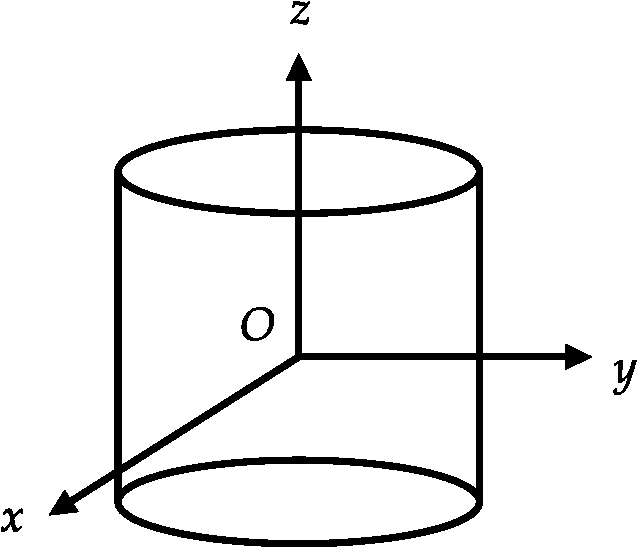
\includegraphics[height=4cm,width=4.5cm]{diagram-20210823(2)-crop}
\end{figure}
\begin{tasks}(4)
	\task[\textbf{A.}] $2 \pi a^{2}(a+h)$
	\task[\textbf{B.}] $3 \pi a^{2} h$
	\task[\textbf{C.}] $2 \pi a^{2} h$
	\task[\textbf{D.}] Zero
\end{tasks}
\item Identify the correct statement for the following vectors $\vec{a}=3 \hat{i}+2 \hat{j}$ and $\vec{b}=\hat{i}+2 \hat{j}$
{\exyear{GATE 2012}}
\begin{tasks}(1)
	\task[\textbf{A.}] The vectors $\vec{a}$ and $\vec{b}$ are linearly independent
	\task[\textbf{B.}] The vectors $\vec{a}$ and $\vec{b}$ are linearly dependent
	\task[\textbf{C.}] The vectors $\vec{a}$ and $\vec{b}$ are orthogonal
	\task[\textbf{D.}] The vectors $\vec{a}$ and $\vec{b}$ are normalized
\end{tasks}
	\item If $\vec{A}$ and $\vec{B}$ are constant vectors, then $\vec{\nabla}(\vec{A} \cdot(\vec{B} \times \vec{r}))$ is
{\exyear{GATE 2013}}

\begin{tasks}(4)
	\task[\textbf{A.}] $\vec{A} \cdot \vec{B}$
	\task[\textbf{B.}] $\vec{A} \times \vec{B}$
	\task[\textbf{C.}] $\vec{r}$
	\task[\textbf{D.}]  Zero
\end{tasks}
\item The unit vector perpendicular to the surface $x^{2}+y^{2}+z^{2}=3$ at the point $(1,1,1)$ is
{\exyear{GATE 2014}}

\begin{tasks}(4)
	\task[\textbf{A.}] $\frac{\hat{x}+\hat{y}-\hat{z}}{\sqrt{3}}$
	\task[\textbf{B.}] $\frac{\hat{x}-\hat{y}-\hat{z}}{\sqrt{3}}$
	\task[\textbf{C.}] $\frac{\hat{x}-\hat{y}+\hat{z}}{\sqrt{3}}$
	\task[\textbf{D.}] $\frac{\hat{x}+\hat{y}+\hat{z}}{\sqrt{3}}$
\end{tasks}
	\item The direction of $\vec{\nabla} f$ for a scalar field $f(x, y, z)=\frac{1}{2} x^{2}-x y+\frac{1}{2} z^{2}$ at the point $P(1,1,2)$ is
{\exyear{GATE 2016}}

\begin{tasks}(4)
	\task[\textbf{A.}] $\frac{(-\hat{j}-2 \hat{k})}{\sqrt{5}}$
	\task[\textbf{B.}] $\frac{(-\hat{j}+2 \hat{k})}{\sqrt{5}}$
	\task[\textbf{C.}] $\frac{(\hat{j}-2 \hat{k})}{\sqrt{5}}$
	\task[\textbf{D.}] $\frac{(\hat{j}+2 \hat{k})}{\sqrt{5}}$
\end{tasks}
\question In spherical polar coordinates $(r, \theta, \phi)$, the unit vector $\hat{\theta}$ at $(10, \pi / 4, \pi / 2)$ is
{\exyear{GATE 2018}}

\begin{tasks}(2)
	\task[\textbf{A.}] $\hat{k}$
	\task[\textbf{B.}] $\frac{1}{\sqrt{2}}(\hat{j}+\hat{k})$
	\task[\textbf{C.}]  $\frac{1}{\sqrt{2}}(-\hat{j}+\hat{k})$
	\task[\textbf{D.}] $\frac{1}{\sqrt{2}}(\hat{j}-\hat{k})$
\end{tasks}
\item Given $\vec{V}_{1}=\hat{i}-\hat{j}$ and $\vec{V}_{2}=-2 \hat{i}+3 \hat{j}+2 \hat{k}$, which one of the following $\vec{V}_{3}$ makes $\left(\vec{V}_{1}, \vec{V}_{2}, \vec{V}_{3}\right)$
a complete set for a three dimensional real linear vector space?
{\exyear{GATE 2018}}

\begin{tasks}(2)
	\task[\textbf{A.}] $\vec{V}_{3}=\hat{i}+\hat{j}+4 \hat{k}$
	\task[\textbf{B.}]  $\vec{V}_{3}=2 \hat{i}-\hat{j}+2 \hat{k}$
	\task[\textbf{C.}] $\vec{V}_{3}=\hat{i}+2 \hat{j}+6 \hat{k}$
	\task[\textbf{D.}] $\vec{V}_{3}=2 \hat{i}+\hat{j}+4 \hat{k}$
\end{tasks}
\end{enumerate}
\colorlet{ocre1}{ocre!70!}
\colorlet{ocrel}{ocre!30!}
\setlength\arrayrulewidth{1pt}
\begin{table}[H]
	\centering
	\arrayrulecolor{ocre}
	\begin{tabular}{|p{1.5cm}|p{1.5cm}||p{1.5cm}|p{1.5cm}|}
		\hline
		\multicolumn{4}{|c|}{\textbf{Answer key}}\\\hline\hline
		\rowcolor{ocrel}Q.No.&Answer&Q.No.&Answer\\\hline
		1&\textbf{a} &2&\textbf{d}\\\hline 
		3&\textbf{b} &4&\textbf{a} \\\hline
		5&\textbf{b} &6&\textbf{d} \\\hline
		7&\textbf{b}&8&\textbf{d}\\\hline
		9&\textbf{d}&10&\textbf{}\\\hline
		
		
	\end{tabular}
\end{table}

\newpage
\begin{abox}
Problem Set-3	
\end{abox}
\begin{enumerate}[label=\color{ocre}\textbf{\arabic*.}]
	\item Three unit vectors $\vec{a}, \vec{b}, \vec{c}\left(\vec{b}\right.$ and $\vec{c}$ are not parallel) are such that $\vec{a} \times(\vec{b} \times \vec{c})=\frac{\sqrt{3}}{2} \vec{c} .$ The
	angles which $\vec{a}$ makes with $\vec{b}$ and $\vec{c},$ respectively are
	\begin{tasks}(2)
		\task[\textbf{a.}]$30^{\circ}, 90^{\circ}$  
		\task[\textbf{b.}]$150^{\circ}, 90^{\circ}$
		\task[\textbf{c.}]$60^{\circ}, 90^{\circ}$ 
		\task[\textbf{d.}]$90^{\circ}, 30^{\circ}$ 
	\end{tasks}
	\begin{answer}
		\begin{flalign*}
		( \vec{a} \times(\vec{b} \times \vec{c})=\frac{\sqrt{3}}{2} \vec{c} &\Rightarrow \vec{b}(\vec{a} \cdot \vec{c})-\vec{c}(\vec{a} \cdot \vec{b})=\frac{\sqrt{3}}{2} \vec{c}
		\intertext{Comparing coefficients of $\vec{b}$ and $\vec{c}$ on both sides.}
		\vec{a} \cdot \vec{c}&=0 \Rightarrow \vec{a} \perp \vec{c}\\
		\vec{a} \cdot \vec{b}&=\frac{\sqrt{3}}{2} \\\Rightarrow a b \cos \theta&=-\frac{\sqrt{3}}{2}\\ \Rightarrow \cos \theta&=-\frac{\sqrt{3}}{2} \\\Rightarrow \theta&=150^{\circ}
		\intertext{The angle which $ \quad\vec{a} $ makes with $ \vec{b}  $ and $ \vec{c} $  are $ 150^{\circ} , 90^{\circ}$ respectively.Correct option is (b)}
		\end{flalign*}
	\end{answer}
\item Find the angle between the two surfaces $5 x+y+z=1$ and $3 x+3 y+3 z=5$.
\begin{tasks}(2)
	\task[\textbf{a.}]$\cos ^{-1}\left(\frac{7}{3}\right)$   
	\task[\textbf{b.}]$\cos ^{-1}\left(\frac{7}{9}\right)$ 
	\task[\textbf{c.}]$\cos ^{-1}\left(\frac{7}{27}\right)$ 
	\task[\textbf{d.}]$\cos ^{-1}\left(\frac{21}{9}\right)$ 
\end{tasks}
\begin{answer}
\begin{align*}
\text{Given}\quad\phi_{1}: 5 x+y+z=1 &\quad\text{and}\quad\phi_{2}: 3 x+3 y+3 z=5\\
\text{therefore,}\\
\cos \theta&=\frac{\vec{\nabla} \phi_{1} \cdot \vec{\nabla} \phi_{2}}{\left|\vec{\nabla} \phi_{1}\right|\left|\vec{\nabla} \phi_{2}\right|}\\&=\frac{(5 \hat{i}+\hat{j}+\hat{k}) \cdot(3 \hat{i}+3 \hat{j}+3 \hat{k})}{\sqrt{27} \cdot \sqrt{27}}\\&=\frac{21}{27} \\\Rightarrow \theta&=\cos ^{-1}\left(\frac{7}{9}\right)
\end{align*}
\end{answer}
\item The equation of the plane that is tangent to the surface $x y z=8$ at the point (1,2,4) is
\begin{tasks}(2)
	\task[\textbf{a.}]$x+2 y+4 z=12$  
	\task[\textbf{b.}]$4 x+2 y+z=12$
	\task[\textbf{c.}]$x+4 y+2=0$ 
	\task[\textbf{d.}]$x+y+z=7$ 
\end{tasks}
\begin{answer}
	\begin{align*}
	\text{To get a normal at the surface let's take the gradient}\\
		\vec{\nabla}(x y z)&=y z \hat{i}+z x \hat{j}+\hat{k} x y\\&=8 \hat{i}+4 \hat{j}+2 \hat{k}\\
		\text{We want a plane perpendicular to this so:}\\
		\left(\vec{r}-\vec{r}_{0}\right) \cdot \frac{(8 \hat{i}+4 \hat{j}+2 \hat{k})}{\sqrt{64+16+4}}&=0\\
		|(x-1) \hat{i}+(y-2) \hat{j}+(z-4) \hat{k}| \cdot[8 \hat{i}+4 \hat{j}+2 \hat{k}]&=0\\ \Rightarrow 4 x+2 y+z&=12
	\end{align*}
	
\end{answer}
\item If $\vec{A}=\hat{i} y z+\hat{j} x z+\hat{k} x y$, then the integral $\oint_{C} \vec{A} \cdot d \vec{l}$ (where $C$ is along the perimeter of a rectangular
area bounded by $x=0, x=a$ and $y=0, y=b)$ is
\begin{tasks}(4)
	\task[\textbf{a.}]$\frac{1}{2}\left(a^{3}+b^{3}\right)$  
	\task[\textbf{b.}]$\pi\left(a b^{2}+a^{2} b\right)$
	\task[\textbf{c.}]$\pi\left(a^{3}+b^{3}\right)$ 
	\task[\textbf{d.}]0 
\end{tasks}
\begin{answer}
	\begin{align*}
	\oint_{C} \vec{A} \cdot d \vec{l}&=\int_{S}(\vec{\nabla} \times \vec{A}) d \vec{a}=0 \\
	\because \vec{\nabla} \times \vec{A}&=0
	\end{align*}

\end{answer}
\item Value of the integral $\oint\left(x y d y-y^{2} d x\right)$, where $c$ is
the square cut from the quadrant by the lines $x=1$ and $y=1$ will be (use Green's theorem to change the line integral into double integral)
\begin{tasks}(4)
	\task[\textbf{a.}] $\frac{1}{2}$ 
	\task[\textbf{b.}]1
	\task[\textbf{c.}]$\frac{3}{2}$ 
	\task[\textbf{d.}]$\frac{5}{3}$ 
\end{tasks}
\begin{answer}
	\begin{align*}
 \intertext{We know that Green's theorem is given by}\oint_{c} \phi d x+\psi d y&=\iint_{R}\left(\frac{\partial \psi}{\partial x}-\frac{\partial \phi}{\partial y}\right) d x d y\\
 \text{Here,}I&=\oint\left(x y d y-y^{2} d x\right)\\&=\oint\left(-y^{2}\right) d x+(x y) d y
 \intertext{Hence, we can deduce}\phi &=-y^{2} \\
 \psi &=x y \\
 \frac{\partial \psi}{\partial x} &=y \\
 \frac{\partial \phi}{\partial y} &=-2 y
 \intertext{Substituting in Green's theorem, we get}
 I &=\int_{y=0}^{1} \int_{x=0}^{1}[y-(-2 y)] d x d y=\int_{y=0}^{1} \int_{x=0}^{1} 3 y d x d y \\
 &=\int_{y=0}^{1}[3 x y]_{x=0}^{1} d y=\int_{y=0}^{1} 3 y d y \\
 &=\frac{3}{2}
\end{align*}
Thus the correct option is (c).
\end{answer}
\item  Evaluate $\int_{C} \vec{F} \cdot \overrightarrow{d r},$ where $F=x^{2} \hat{i}+y^{3} \hat{j}$ and curve $C$ is the arc of parabola $y=x^{2}$ in the $x-y$
plane from (0,0) to (1,1) 
\begin{tasks}(2)
	\task[\textbf{a.}]$\frac{7}{12}$  
	\task[\textbf{b.}]$\frac{7}{12}$ 
	\task[\textbf{c.}]$\frac{7}{12}$  
	\task[\textbf{d.}]$\frac{7}{12}$ 
\end{tasks}
\begin{answer}
	\begin{align*}
	\text{Along the curve C,}
	y=x^{2} \Rightarrow d y=2 x d x ;\\
	\vec{r}&=x \hat{i}+x^{2} \hat{j} \Rightarrow d \vec{r}=d x \hat{i}+2 x d \hat{x} j\\
	\text { Therefore, } \int_{C} \vec{F} \cdot d \vec{r}&=\int_{x=0}^{1}\left[x^{2} d x+x^{6}(2 x) d x\right] \\
	&=\int_{0}^{1}\left(x^{2}+2 x^{7}\right) d x=\left[\frac{x^{3}}{3}+\frac{2 x^{8}}{8}\right]_{0}^{1}\\&=\frac{7}{12}
	\end{align*}
	
\end{answer}
\item At any point of the curve $x=3 \cos t, y=3 \sin t, z=4 t,$ find
The unit tangent vector 
\begin{tasks}(2)
	\task[\textbf{a.}]$\frac{1}{\sqrt 10}(-3 \sin t \hat{i}+3 \cos t \hat{j}+4 \hat{k})$   
	\task[\textbf{b.}]$\frac{1}{10}(-3 \sin t \hat{i}+3 \cos t \hat{j}+4 \hat{k})$ 
	\task[\textbf{c.}]$\frac{1}{5}(-3 \sin t \hat{i}+3 \cos t \hat{j}+4 \hat{k})$ 
	\task[\textbf{d.}]$\frac{1}{5(\sin t+\cos t)}(-3 \sin t \hat{i}+3 \cos t \hat{j}+4 \hat{k})$  
\end{tasks}
\begin{answer}
\begin{align*}
	\quad\vec{r} &=x \hat{i}+y \hat{j}+z \hat{k} \Rightarrow \vec{r}=(3 \cos t) \hat{i}+(3 \sin t) \hat{j}+(4 t) \hat{k} \\
	\frac{d \vec{r}}{d t} &=(-3 \sin t) \hat{i}+(3 \cos t) \hat{j}+4 \hat{k}\quad
	\text{which is the required tangent vector.} \intertext{Magnitude of tangent vector} &=\sqrt{(-3 \sin t)^{2}+(3 \cos t)^{2}+(4)^{2}}=5
	\intertext{Unit tangent vector}&=\frac{1}{5}(-3 \sin t \hat{i}+3 \cos t \hat{j}+4 \hat{k})
\end{align*}
\end{answer}
\item The unit normal vector of the point $\left[\frac{a}{\sqrt{3}}, \frac{b}{\sqrt{3}}, \frac{c}{\sqrt{3}}\right]$ on the surface of the ellipsoid
$\frac{x^{2}}{a^{2}}+\frac{y^{2}}{b^{2}}+\frac{z^{2}}{c^{2}}=1$ is
\begin{tasks}(2)
	\task[\textbf{a.}]$\frac{b c \hat{i}+c a \hat{j}+a b \hat{k}}{\sqrt{b^{2} c^{2}+c^{2} a^{2}+a^{2} b^{2}}}$  
	\task[\textbf{b.}]$\frac{a \hat{i}+b \hat{j}+c \hat{k}}{\sqrt{a^{2}+b^{2}+c^{2}}}$
	\task[\textbf{c.}]$\frac{b \hat{i}+c \hat{j}+a \hat{k}}{\sqrt{a^{2}+b^{2}+c^{2}}}$ 
	\task[\textbf{d.}]$\frac{\hat{i}+\hat{j}+\hat{k}}{\sqrt{3}}$ 
\end{tasks}
\begin{answer}
	\begin{align*}
	\text{Here,}\phi&=\frac{x^{2}}{a^{2}}+\frac{y^{2}}{b^{2}}+\frac{z^{2}}{c^{2}}-1\\
	\text{Unit normal vector is}\frac{\vec{\nabla} \phi}{|\vec{\nabla} \phi|}\\
	\text{So}\vec{\nabla} \phi&=\left(i \frac{\partial}{\partial x}+\hat{j} \frac{\partial}{\partial y}+\hat{k} \frac{\partial}{\partial z}\right) \cdot\left(\frac{x^{2}}{a^{2}}+\frac{y^{2}}{b^{2}}+\frac{z^{2}}{c^{2}}-1\right)\\&=\frac{2 x \hat{i}}{a^{2}}+\frac{2 y \hat{j}}{b^{2}}+\frac{2 z \hat{k}}{c^{2}}\\
	\left.\vec{\nabla} \phi\right|_{\left(\frac{a}{\sqrt{3}}, \frac{b}{\sqrt{3}}, \frac{c}{\sqrt{3}}\right)}&=\frac{2}{a \sqrt{3}} \hat{i}+\frac{2}{b \sqrt{3}} \hat{j}+\frac{2}{c \sqrt{3}} \hat{k}\\
	|\vec{\nabla} \phi|&=\sqrt{\frac{4}{3 a^{2}}+\frac{4}{3 b^{2}}+\frac{4}{3 c^{2}}}\\&=\frac{2}{\sqrt{3}} \sqrt{\frac{b^{2} c^{2}+a^{2} c^{2}+a^{2} c^{2}}{a^{2} b^{2} c^{2}}}\\
	\left.\frac{\vec{\nabla} \phi}{|\vec{\nabla} \phi|}\right|_{\left(\frac{a}{\sqrt{3}}, \frac{b}{\sqrt{3}}, \frac{c}{\sqrt{3}}\right)}&=\frac{\frac{2}{a \sqrt{3}} \hat{i}+\frac{2}{b \sqrt{3}} \hat{j}+\frac{2}{c \sqrt{3}} \hat{k}}{\frac{2}{\sqrt{3}} \frac{\sqrt{b^{2} c^{2}+c^{2} a^{2}+a^{2} b^{2}}}{a b c}}\\&=\frac{b c \hat{i}+c a \hat{j}+a b \hat{k}}{\sqrt{b^{2} c^{2}+c^{2} a^{2}+a^{2} b^{2}}}
	\end{align*}
The correct option is (a)
\end{answer}
\item For the vector field $\vec{A}=x z^{2} \hat{i}-y z^{2} \hat{j}+z\left(x^{2}-y^{2}\right) \hat{k},$ the volume integral of the divergence of $\vec{A}$
out of the region defined by $-a \leq x \leq a,-b \leq y \leq b$ and $0 \leq z \leq c$
is:
\begin{tasks}(2)
	\task[\textbf{a.}]$\frac{4}{3} a b c\left[a^{2}-b^{2}\right]$  
	\task[\textbf{b.}] $\frac{2}{3} a b c\left[a^{2}-b^{2}\right]$
	\task[\textbf{c.}]$\frac{1}{3} a b c\left[a^{2}-b^{2}\right]$ 
	\task[\textbf{d.}]$a b c\left[a^{2}-b^{2}\right]$ 
\end{tasks}
\begin{answer}
	\begin{align*}
	\text{Since,} \vec{A}&=x z^{2} \hat{i}-y z^{2} \hat{j}+z\left(x^{2}-y^{2}\right) \hat{k} \Rightarrow \vec{\nabla} \cdot \vec{A}=z^{2}-z^{2}+\left(x^{2}-y^{2}\right)=x^{2}-y^{2}\\
	\text{Thus,}\int_{V}(\vec{\nabla} \cdot \vec{A}) d \tau\\&=\int_{x=-a}^{x=+a} \int_{y=-b}^{y=+b} \int_{z=0}^{z=c}\left(x^{2}-y^{2}\right) d x d y d z\\&=\int_{y=-b}^{y=+b} \int_{z=0}^{z=c}\left[\frac{x^{3}}{3}-y^{2} x\right]_{-a}^{+a} d y d z\\&=\int_{y=-b}^{y=+b} \int_{z=0}^{z=c}\left[\frac{2}{3} a^{3}-2 a y^{2}\right] d y d z\\
	\Rightarrow \int_{V}(\vec{\nabla} \cdot \vec{A}) d \tau&=\int_{z=0}^{z=c}\left[\frac{2}{3} a^{3} y-2 a \frac{y^{3}}{3}\right]_{-b}^{+b} d z=\int_{z=0}^{z=c}\left[\frac{4}{3} a^{3} b-\frac{4}{3} a b^{3}\right] d z\\&=\frac{4}{3} a b c\left[a^{2}-b^{2}\right]
	\end{align*}
 Correct option is (a)
\end{answer}
\item The value of $\oint \vec{F} \cdot d \vec{r},$ where $C$ is the curve bounded by $x^{2}+y^{2} \geq 4 ; x^{2}+y^{2} \leq 16 ; x \geq 0$
and $\vec{F}=-y \hat{i}+x \hat{j}+z \hat{k}$ is ....
\begin{tasks}(4)
	\task[\textbf{a.}]$ 12\pi$ 
	\task[\textbf{b.}]$ 24 \pi$ 
	\task[\textbf{c.}]$ \frac{14 \pi}{3}$  
	\task[\textbf{d.}]$ \frac{10 \pi}{3}$  
\end{tasks}
\begin{answer}
\begin{align*}
\intertext{Using Stoke's theorem,}\int_{C} \vec{F} \cdot d \vec{r}&=\iint_{S}(\vec{\nabla} \times \vec{F}) \cdot d \vec{S}\\
\int_{C} \vec{F} \cdot d \vec{r}&=\iint_{S}(\vec{\nabla} \times \vec{F}) \cdot d \vec{S}\\
\vec{\nabla} \times \vec{F}&=\left|\begin{array}{ccc}
\hat{i} & \hat{j} & \hat{k} \\
\frac{\partial}{\partial x} & \frac{\partial}{\partial y} & \frac{\partial}{\partial z} \\
-y & x & z
\end{array}\right|=\hat{i}(0-0)-\hat{j}(0-0)+\hat{k}(1+1)=2 \hat{k}\end{align*}
\begin{figure}[H]
	\centering
	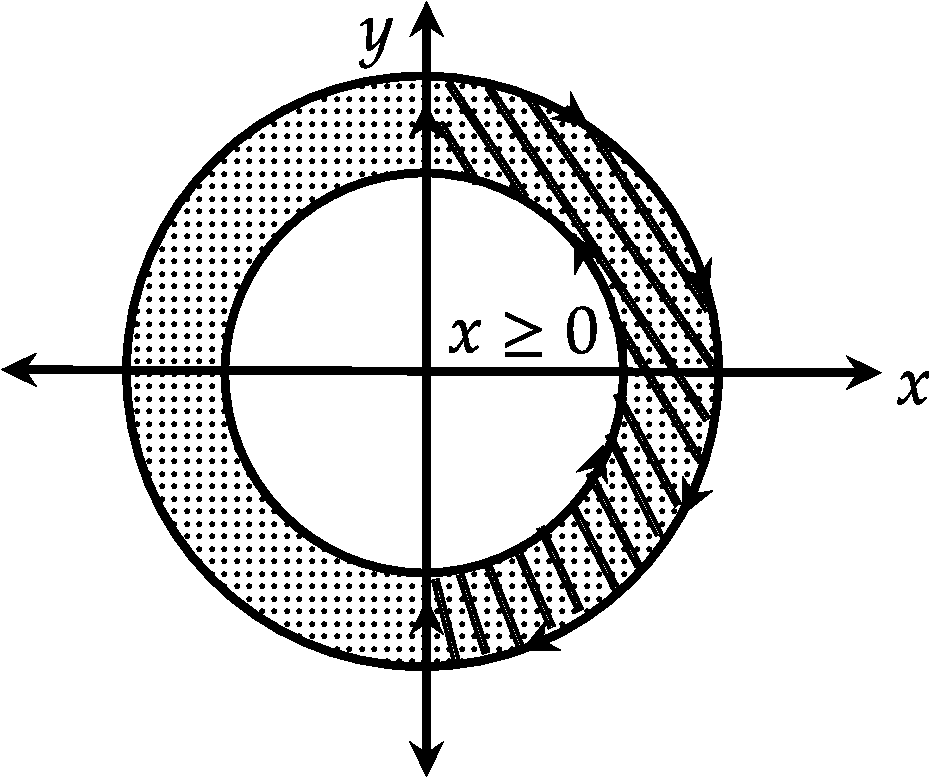
\includegraphics[height=3.5cm,width=4cm]{pset 3-10}
\end{figure}
\begin{align*}
\text { And } d \vec{S}&=d x d y \hat{k}\\
\therefore \quad \iint_{S}(\vec{\nabla} \times \vec{F}) \cdot d \vec{S}&=2 \iint d x d y\\
\intertext { Put, $ x=r \cos \theta, y=r \sin \theta $  and  $ d x d y=r d r d \theta $}
&=2 \int_{\theta=-\frac{\pi}{2}}^{\frac{\pi}{2}} \int_{r=2}^{4} r d r d \theta\\&=2\left(\frac{r^{2}}{2}\right)_{2}^{4}( \pi)= \pi \times 12=12 \pi
\end{align*}	
\end{answer}

\end{enumerate}


